\documentclass[a4Paper,12pt]{report}
\usepackage[margin=1.0in]{geometry}
\usepackage{newtxtext,newtxmath}
\usepackage{fancyhdr}  
\usepackage{tabularx}
\usepackage{caption}
\usepackage{graphicx}
\usepackage{float}
\usepackage{hyperref}
\usepackage{cite}
\usepackage{natbib}
\bibliographystyle{plainnat}
\captionsetup[table]{justification=centering}
\captionsetup[figure]{justification=centering}
\parindent 0px

\fancyhf{}
\lhead{\fancyplain{}{\textit{\nouppercase{\textbf{\leftmark}}}}}
\rhead{\fancyplain{}{\textbf{\thepage}}}

\begin{document}
\begin{titlepage}
\begin{center}

\includegraphics[scale=0.1]{images/a_and_s_logo.png}\\[1cm]
	\begin{Huge}
	INDIVIDUAL ASSIGNMENT ONE REPORT
	\end{Huge}\\[1cm]
    \begin{Large}
    LEVEL 6
    \end{Large}\\[0.5cm]
    \begin{Large}
    COMP60022
    \end{Large}\\[1cm]
    \begin{huge}
    DECISION ANALYTICS
    \end{huge}\\[0.5cm]
    \begin{LARGE}
    HFK2422COM HFK2422COMF
    \end{LARGE}\\[1cm]
    \begin{large}
    Hand Out Date: 28/07/2024
    \end{large}\\[0.5cm]
    \begin{large}
    Hand In Date: 07/10/2024
    \end{large}\\[1cm]
    \hrule
    \vspace{1cm}
    \begin{center}
    \begin{tabular}{rll}\hline
    \textbf{Staffordshire Student Number} & \textbf{Student CB Number} & \textbf{Student Full Name}\\\hline
     21035795 & CB010406 & Kavinda Kethiya Rajapaksha\\\hline
    \end{tabular}
    \end{center}
    \vspace{1cm}
    \hrule
\end{center}
\end{titlepage}
\tableofcontents
\listoftables
\listoffigures
\pagestyle{fancyplain}
\chapter{Introduction}
\section{Problem Context Status}
Nexart is an enterprise which manufactures and sells networking devices and accessories to clients. This enterprise was started in 2000 by Alexander Watson. Nexart branches are located all around the globe and the main branch is situated in California, USA.
\begin{figure}[H]
\centering

\includegraphics[scale=0.4]{images/nexart_trademark.png}
\caption{Nexart Enterprise Logo}
\end{figure}
\begin{figure}[H]
\centering
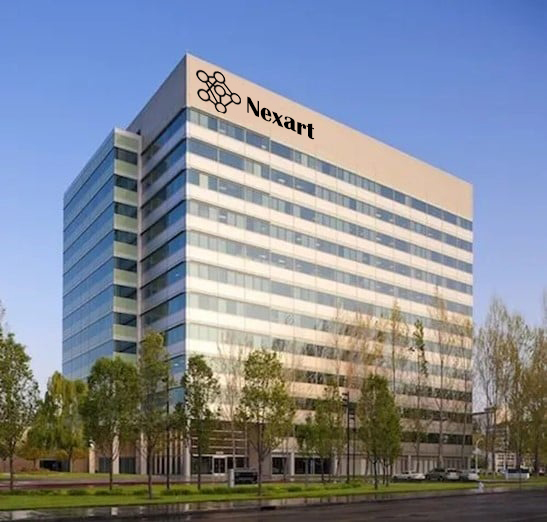
\includegraphics[scale=0.4]{images/nexart_office.jpg}
\caption{Nexart Head Office California}
\end{figure}
\begin{figure}[H]
\centering
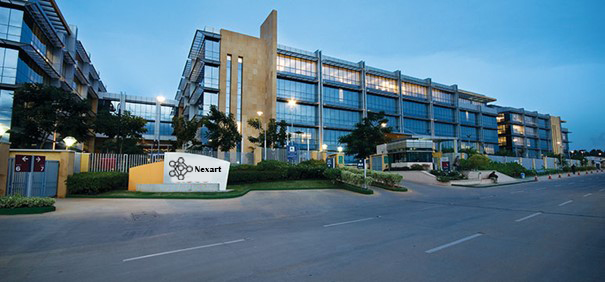
\includegraphics[scale=0.8]{images/nexart_production_plant.jpg}
\caption{Nexart Production Plant California}
\end{figure}
Manufactured devices and accessories are distributed to Nexart subbranches of other nations via shipping according to the requests of subbranches. Network infrastructure installation companies play the role of Nexart clients. They provide services to government and non-government organizations. After getting quotations approved from the clients, they place orders by logging onto Nexart website. The clients choose their nearest Nexart branch and select the network equipment that they require for the job and proceed to make payments. They fill out the payment details and finalize the payment. Nexart send an email to the client informing about the order that the customer has placed, and the order details include payment amount and network equipment details. In addition, Nexart also provide shipping details and order tracking details in the mail. So that the clients can keep track of the orders. Each of the Nexart subbranches have a stock. When they are out of stock, they order items from their nearest subbranch. In this manner, Nexart optimize their shipping costs. In comparison to past years, the revenue of Nexart has skyrocketed drastically.\\[12pt]
Nexart enterprise uses the relational database management system, Microsoft SQL Server to store the records of clients, branches, products, orders, and stock requests. The attributes inherited by the client entity are client id, name, contact information, billing address and registered date. Features inherited by the branch are branch id, name, location, contact information and stock. Device object is inherited by the product id, name, description, and price. The characteristics owned by the order entity are order id, order date, total amount, items, payment, and shipping. The attributes which belong to the Stock Request are stock request id, request date and quantity requested. As the customer base of the Nexart grew rapidly, the databases were unable to handle the requests from clients all around the globe. This resulted in latencies in database operation, lack of interest in customers, losing business edge, increased expenses and under performance of businesses. Apart from the business impacts, the Nexart also suffers from scalability, query latencies, concurrency limits, cost efficiency and schema rigidity issues. Complexity issues and errors have occurred due to maintaining integrity and maintenance. So, the Nexart clients were not satisfied with the service, and they turned towards their main competitor Cisco. This resulted in a revenue decline, and they had to plead with customers to purchase items from them. The CEO of Nexart wanted to get things back on track and he escalated the issue to the IT Department. The data engineers of the IT department started to narrow down issues step by step, isolating irrelevant factors. This process is discussed thoroughly in the next section.
\section{Business Questions}
Data engineers assess the allegations of their clients regarding the web application. With the corporation of network engineers, they monitor network traffic. According to the observation, they noticed that the increase of their clients compared to past. In addition, they notice that Nexart generates bulks of data compared to past. As they produce new network devices and accessories for the market, new features are added to the device table. This results in storage expansion and order processing delays were caused due to the number of queries that I have been fired towards the MSQL database during peak hours. Nexart did not encounter this issue before because of the lower customer base and limited devices on the production line. The issue can be assessed with the following questions.
\begin{itemize}
\item What factors caused the revenue loss? 
\item Why did the revenue decline occur?
\item Where did the revenue decline occur? 
\item When did the revenue decline occur? 
\item Who is part of the revenue decline? 
\item What are the measures that can be taken to enhance the accuracy of real-time data processing and downsize query latency? 
\item How much expenditure can be saved from migrating all the data that is in the MSSQL to MongoDB database? 
\item What actions can be taken to manage data storage effectively in terms of scaling data? 
\item How does the database can manage the real-time sensor data that is being generated in production? 
\item How to ensure redundant connectivity to the database as the number of users grows?
\item How does the latencies in query responses can affect customer satisfaction?
\end{itemize}
Every bit of data generated by the Nexart may possess a value. So, it would be unwise to get rid of the data without accurately assessing it. The next chapter discusses the ways of managing Nexart’s generated data in an effective manner.
\chapter{Databases}
\section{Concepts}
Nexart stores their daily generated data in a database before processing it in a database. Organized data stored as soft copies in a computer is defined as a database. To manage a database, a Database Management System is required.\\[12pt]
They are categorized into two categories, and they are Relational, Non-Relational, NewSQL, InMemory, Time-Series and Object-oriented Databases. NewSQL database is considered as an enhanced version of a relational database. Scalability acts as the icing for these databases. Google Spanner and CockraochDB are examples for NewSQL databases. Main memory is used by Memory databases to store data. Perfect instances for NewSQL databases are Redis and Memcached. Data generated by IoT devices and financial transactional data are stored in Time-Series databases and time stamped. InfluxDB and TimeScaleDB are examples of TimeSeries databases. Data are stored as objects in Object-Oriented databases.db40 and ObjectDB are instances for Object-Oriented Databases.\\[12pt]
Single-Tier, Two-Tier, Three-Tier and N-Tier are database Architectures. In a Single-Teir architecture, the database and application are hosted in the same machine and deployed in development/testing environments. Direct communication between the client and the server is maintained in a Two-Tier architecture and its applications are applications which fall in the range of small to medium. An intermediary layer is added to enhance the capabilities of a Three-Teir architecture, and they are used in web applications, enterprise applications etc. As an enhancement Three-Tier designs add an intermediary layer. N-Tier architecture is used to address complex commercial issues that are related to databases. This architecture surpasses the third architecture by adding more layers. Mostly conglomerate applications use N-Tier architecture for their systems.\\[12pt]
The components of the database are Database Engine, Database Schema, Query Processor, Storage Manager, Transaction Manager, Concurrency Control Manager and Recovery Manager. The Database Engine is responsible for accessing and managing the database and this service is considered a core service. The Logical structure of a database is defined as the Logical Schema of a database and it includes tables, views etc. The mechanism which is responsible for interpreting and executing queries is the Query Selector. The storage manager plays the role of managing the disk space. The transaction manager makes sure that all the transactions happen according to the properties of ACID. The consistency of simultaneous data access is managed by the concurrency control manager. When a database failure occurs, the recovery manager restores the database back to its normal condition.\\[12pt]
According to the design aspect of databases, they can be divided into three categories, and they are Conceptual Design, Logical Design and Physical Design. A perfect example for a conceptual design would be entity relationship diagrams. These diagrams illustrate the data model. The Logical Design demonstrates the database in the form of tables, views etc.\\[12pt]
To avoid redundancies and enhance data integrity normalization is carried out. 1st, 2nd, 3rd, and 4th normalization are examples of normalization types.\\[12pt]
The data are efficiently retrieved by using the database indexing mechanism. Primary, secondary, clustered, and non-clustered indexing are instances for database indexes. Authentication, Authorization, Encryption and Backup and Recovery mechanisms take care of the security just in case of a security breach. Authentication is responsible for verifying the identity of the user while the actions that the verified user can perform are granted by authorization. Encryption mechanism encrypts the data using hashing algorithms before storing or transporting them in the database. Backup and recovery mechanisms make sure that the data can be restored back to its normal condition in case of data loss or corruption. Full back up, incremental backup and differential backup are examples for database backup methods. The entire database is copied to a storage device in full backup method. Incremental backups copy the recently altered data to a storage device. The data changed since the last full backup is copied to a storage device in differential backup method. Restoring data to a certain point in time is defined as point-in-time recovery. Recovering recently committed data by examining the transaction logs is part of the log-based recovery method. Cloud, Distributed and Graph databases are considered as modern trends of databases.\\[12pt]
The accurate processing of database transactions is assured by the properties of ACID and their atomicity, consistency, isolation, and durability. A transaction is treated as a one unit in Atomicity while all the standards are maintained under consistency. Isolation mechanism compartmentalizes each transaction until they terminated. Fault tolerances in transactions are ensured by the durability property. The next section draws out the advantages and disadvantages of relational and non-relational databases.
\section{Relational and Non-Relational Databases}
Structured data are stored in relational databases using columns and rows while semi-structured and unstructured data are stored in non-relational databases. Structured Query Language is used by relational databases to perform all the database operations while Not Structured Query Language is used by non-relational databases to perform all the database operations. MySQL, PostgresSQL, Oracle and SQL Server are examples of relational databases. There are four types of non-relational databases, and they are Document Stores, Key-Value Stores, Column Stores and Graph Databases. MongoDB and CouchDB are examples for Document Stores while Redis and DynamoDB are instances for Key-Value Stores. Cassandra and HBase are examples for column store NOSQL databases. Neo4j and ArangoDB are the best examples for graph databases. The table below highlights the main differences between SQL and NOSQL.
\begin{table}[H]
\centering
\begin{tabularx}{\textwidth}{XX}\hline
SQL & NOSQL\\\hline
Used in relational databases & Used in non-relational databases\\
Has static schema design and structure & Has dynamic schema design and structure\\
Handle complex queries & Handle large volumes of data\\
Equipped with vertical scalability & Equipped with horizontal scalability\\
Follows ACID property & Follows CAP property\\\hline
\end{tabularx}
\caption{Pros and Cons of SQL and NOSQL}
\end{table}
Relational and non-relational databases such as MSSQL and MongoDB have ACID in common. Though a transaction is complete or rolled back, atomicity ensures that the database is maintained in a consistent state in MSSQL. Atomicity is applied in a single document update process in MongoDB. Constraints, triggers, and rule mechanisms ensure that consistency is maintained in MSSQL. Consistency is applied for multi-documents in MongoDB, and it is offered via flexible schema design which enables read and write operations. Transparency of uncommitted changes to other transactions is maintained via isolation mechanism in MSSQL. Snapshot mechanism in MongoDB ensures isolation in multi-document transactions. Transactions logs and database backups ensure that durability is maintained in MSSQL while journaling and replica sets ensure durability In MongoDB. The benefits and drawbacks of relational and non-relational databases are discussed in the next section.
\section{Strength and Weaknesses of Relational and Non-Relational Databases}
The table given below spotlights the pros and cons of relational databases.
\begin{table}[H]
\centering
\begin{tabularx}{\textwidth}{XX}\hline
Advantages & Disadvantages\\\hline
Provides a structure to manage data & Limited Scalability\\
Compatible with ACID & Performance issues\\
Extensive Query Capabilities & Difficulty in changing the schema\\
Avoiding data redundancy and enhancing data integrity & High Cost\\
Capability of mapping complex relationships between entities & Difficulties in handling semi-structured and unstructured data\\
Technical Support & Complexity in applications\\
Security & Unability of handling datasets that scaling.\\\hline
\end{tabularx}
\caption{Advantages and Disadvantages Relational Databases}
\end{table}
The advantages and disadvantages of non-relational databases are emphasized in the table given below.
\begin{table}[H]
\centering
\begin{tabularx}{\textwidth}{XX}\hline
Advantages & Disadvantages\\\hline
Scalability & Not Consistent\\
Availability & Consistency Issues\\
Higer Performance & Limited Query Capabilities\\
Flexibility & ACID not supported\\
Handling of structured and unstructured data & Limited support\\
Low Expenditure & Complexity in terms of data modeling\\\hline
\end{tabularx}
\caption{Benifits and Drawbacks of Non-Relational Databases}
\end{table}
We have already acknowledged the benefits and drawbacks of relational and non-relational databases. Next step would be to select the right database type for your application and the next chapter addresses about it.
\section{Right Database Option for an application}
Applications use relational or non-relational databases to store data according to the project requirements. As we acknowledged before, relational, and non-relational databases use SQL and NOSQL to perform all database operations. If an application has structured data with a static schema and requires multirow transactions, it is advisable to deploy a relational database such as MSSQL. The developers still can go with non-relational databases, but it can limit the functionality of the application sometimes. It may take a toll on the project budget sometimes. If a solution has a dynamic schema and holds semi-structured and unstructured data, it would be ideal to use a non-relational database such as MongoDB. The characteristic of a non-relational database supports an enterprise application which is scaling at a rapid rate. A relational database can be used for this application, but it will downgrade the capabilities of the application even if the option is less costly. NOSQL databases are ideal for solutions which require hierarchical storage structures, scalable features, and functions and where relationships between entities are not important. Maintenance of a database is important for an application to run smoothly without causing any issues. Operations such importing and exporting data occur in the management phase. Hence these tasks are repetitive, automation is required to boost the system's productivity. The next chapter suggests an enhancement to improve the efficiency of the Nexart system.
\chapter{Data Engineering}
\section{Data Engineering Concepts}
CTO of Nexart decided to merge Data Science capabilities, Machine Learning and AI with their generated data to increase revenue and to anticipate future revenue losses of the organization. AI’s are empowered with quality data. Machine Learning algorithms analyze data and make predictions. The principles of Data Engineering guide in the Data Analysis processes. Data Science and Data Engineering fields have common characteristics. The picture given below demonstrates aspects in IT where data science is applied.
\begin{figure}[H]
\centering
\fbox{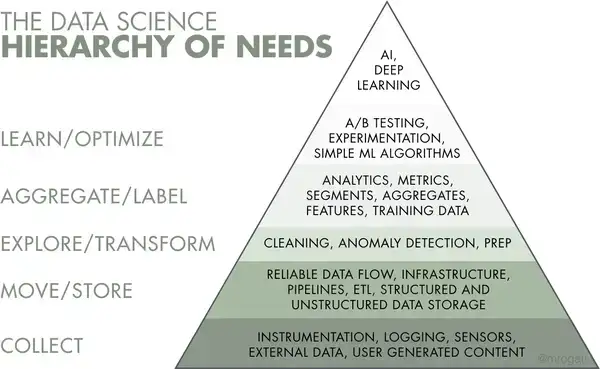
\includegraphics[scale=0.7]{images/data_science.png}}
\caption{Hierarchy of Data Science Necessities}
\end{figure}
The data engineers of Nexart gather generated data from departments and store in the MongoDB database for data scientists, data analysts, business intelligence developers and other IT specialists within the Nexart to access at any time. They chose the MongoDB database due to its scalability. The image given below demonstrates the steps that are followed in the data engineering process. 
\begin{figure}[H]
\centering
\fbox{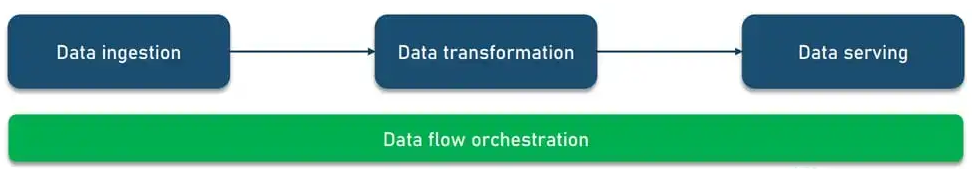
\includegraphics[scale=0.5]{images/data_engineering.png}}
\caption{Data Engineering Processes}
\end{figure}
All the collected data from Nexart Departments will be moved to MongoDB database in the data ingestion state. In the data transformation stage, highly demandable data will be cleaned, normalized, and converted to the required format. The users of Nexart that requested data will be served with data in the data serving process. The transparency of data engineering process is maintained through data flow orchestration. This gives the privilege of monitoring data workflows and repairing data quality and performance issues. Automating the steps followed in the data engineering process is defined as a data engineering pipeline. Data from the MSSQL database is moved to MongoDB database with the aid of data engineering pipelines by coupling tools with operations. In addition, data engineers of Nexart could write a script to get weekly/monthly/yearly sales reports. Hence the generation of sales reports is a repetitive task.\\[12pt]
Since Nexart enterprise is dealing with big data, the data engineers decided to go with a big data engineering pipeline that uses ELT method. The image below captures the whole ELT process.
\begin{figure}[H]
\centering
\fbox{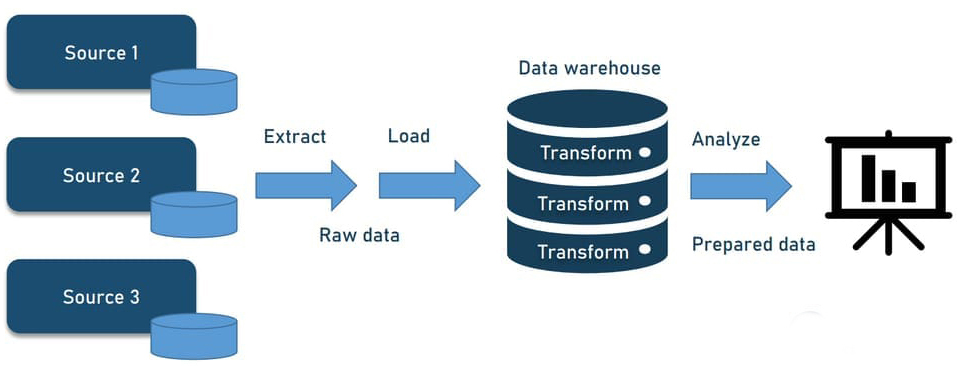
\includegraphics[scale=0.5]{images/elt_pipeline.jpg}}
\caption{ELT Pipeline}
\end{figure}
ETL functions differently compared to ELT pipelines. We can observe the functionality of ETL from the image given below.
\begin{figure}[H]
\centering
\fbox{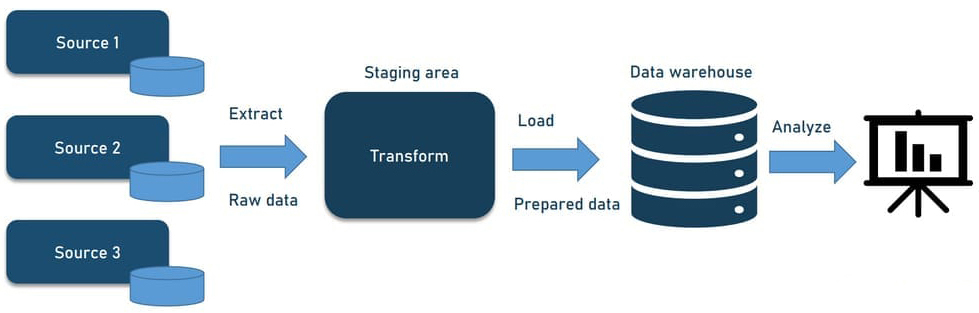
\includegraphics[scale=0.5]{images/etl_pipeline.jpg}}
\caption{ETL Pipeline}
\end{figure}
Apart from data migrations, Nexart can deploy the pipeline for data wrangling, data integration and copying databases. A data pipeline consists of 7 components, and they are origin, destination, dataflow, storage, processing, workflow, and monitoring. MSSQL and MongoDB play the role of source and destination, respectively. The dataflow defines changes that data undergoes from the source to the destination. As data moves from MSSQL to MongoDB, the data will be stored in the lake.
\begin{figure}[H]
\centering
\fbox{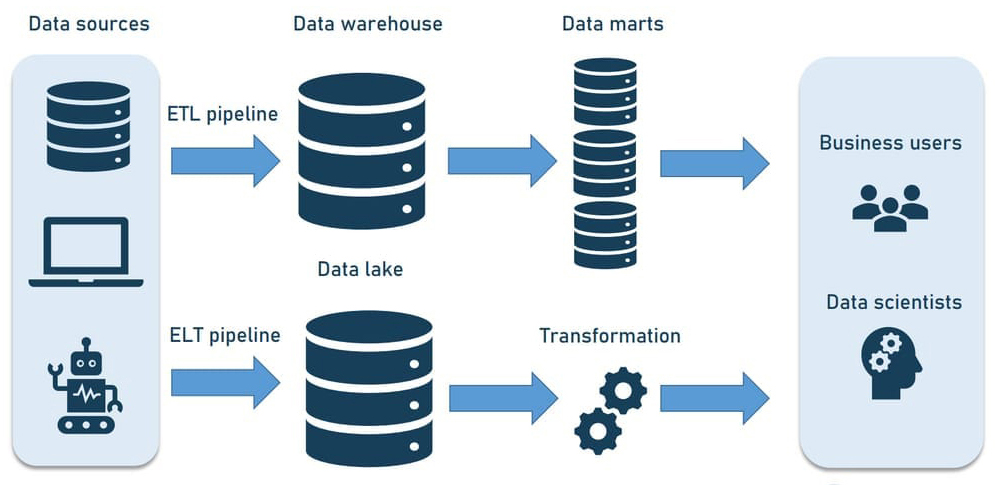
\includegraphics[scale=0.5]{images/big_data.jpg}}
\caption{Data Lake with Big Data Infrastructure}
\end{figure}
Processing defines the ingestion, storing and transformation of data from the source to the destination. The workflow defines a set of activities that are carried out from the Source to the destination, and it also highlights dependencies that each task has on them. The monitoring mechanism ensures the data is in proper shape. It would be ideal for Nexart to maintain two data pipelines. One pipeline should follow batch processing while the other should stream processing. In some instances, Nexart would have to investigate old records to make a business decision and sometimes the corporation would have to deal with real-time data such as data generated from robots on the production line. So, in this case it is better to maintain two data pipelines. \\[12pt]
Data pipeline tools branches under ELT, Data Warehousing, Data Lake, Batch Work-flow Schedulers, Real-Time Data Streaming and Big Data tools. All the data preparation and integration tools fall under ETL tools and IBM DataStage Informatica power Center, Oracle Data Integrator, Talend Open Studio are examples for ETL tools. Instances for Data Warehouse tools are Amazon Redshift, Azure Synapse, Google BigQuery, Snowflake and Teradata. AWS, Microsoft Azure, Google Cloud, and IBM are examples of cloud service providers which offer data lakes as tools. Luigi and Azkaban are batch workflow schedulers which declare tasks programmatically along with their dependencies. In addition, they have the capability of monitoring and automating the tasks. Apache Kafka, Apache Storm, Google Data Flow, Amazon Kinesis, Azure Stream Analytics, IBM Streaming Analytics and SQL Stream are tools that are used process real-time data that are generated by machine sensors, IoT sensors etc \cite{alexsoft}. The data pipeline tools mentioned do not go well with Big Data. The software developers have developed specific tools to perform heavy duty operations such as prepping data pipelines for big data. Let us review each of these tools. Hadoop and Spark platforms are used for batch processing big data. The Spark streaming analytics service tool enhances the functionality of the Spark platform. Apache Oozie and Apache Airflow tools are used by data engineers to perform scheduling and monitoring for batch jobs. Cloud service providers such as Amazon, Google, IBM, Microsoft, and Alibaba offer their own tools for data experts to create big data pipelines. As we have acknowledged the DNA of data engineering, the next segment discusses how the principles of data engineering are applied towards the Nexart case study. 
\section{Data Engineering Pipeline}
As we acknowledged before Nexart decided to go with the ELT method for both data pipelines. The data engineers of Nexart are not sure about the way of transforming data and they have an idea of generating insights into the future as well. Due to these reasons, they decided to go with the ELT method. Since Nexart is generating tons of data daily from the production line and other departments, they decided to go with tools that are specifically designed for big data. Let us discuss the data pipelines further.\\[12pt]
To increase the revenue, Nexart needs valuable insights from data that been stored in the MSSQL database. These insights are being generated using machine learning. Models need to be fed loads of data to get better insights. So, the model requires processed data from the past and the present and they decided to go with a batch processing data pipeline to get business insights. Apache NiFi, MongoDB, Apache Spark, and Airflow tools will be used for the batch processing data pipeline. In this pipeline there are three phases. Data stored in the MSSQL database needed to be extracted firsthand. Before commencing the first phase, the system engineers of Nexart will determine the peak hours of service by analyzing incoming and outgoing traffic of Nexart. After that the data engineers of Nexart will extract data from MSSQL database according to off peak hours defined by the data engineer using Apache NiFi software.\\[12pt]
\begin{figure}[H]
\centering
\fbox{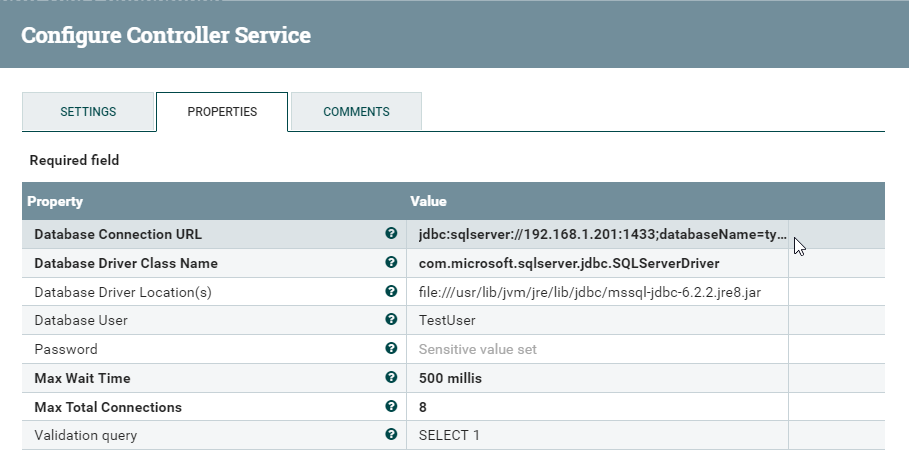
\includegraphics[scale=0.4]{images/data_extraction.png}}
\caption{Apache NiFi Extracting Data From MSSQL Database}
\end{figure}
This application gives the privilege of setting up data extraction schedules. As a plus point this does not clash the ongoing services of Nexart during peak hours. Extracted data will be needed to store in a storage.\\[12pt]
\begin{figure}[H]
\centering
\fbox{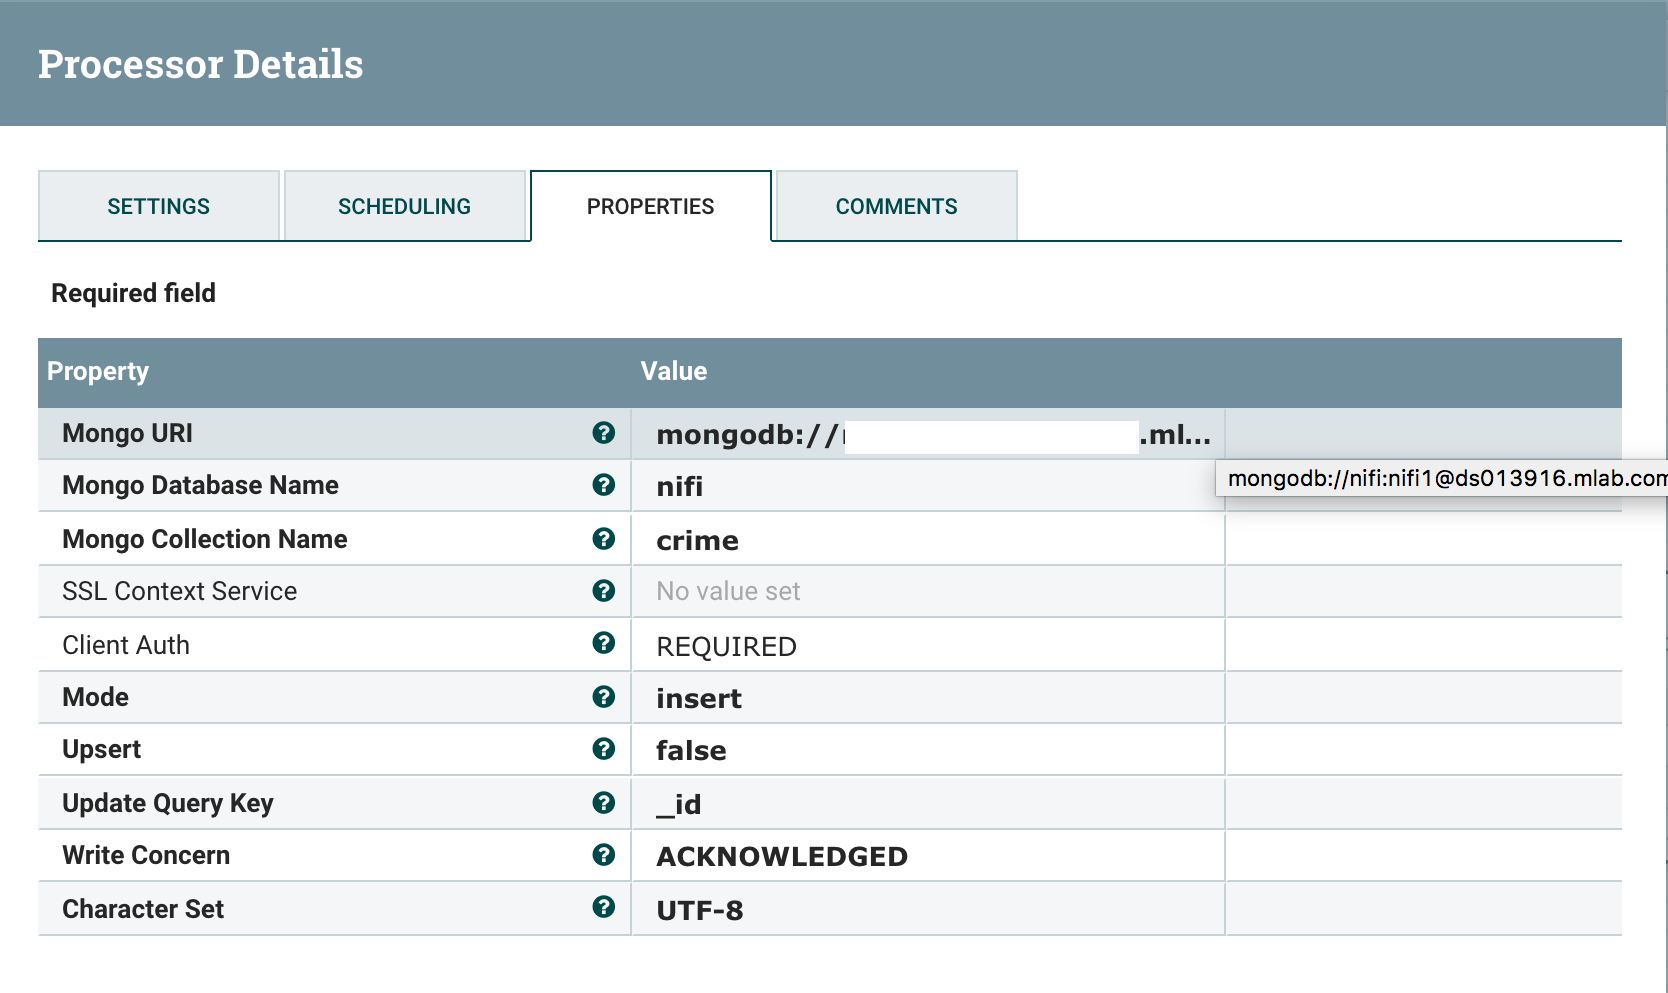
\includegraphics[scale=0.2]{images/data_storing.png}}
\caption{Apache NiFi Storing Extracted Data in MongoDB Database}
\end{figure}
The schemeless characteristic of MongoDB database addresses the storage problem by storing all extracted raw data from MSSQL database. This enables us to maintain the integrity of data. This raw data does not have a meaning. So, these data needed transformed to get a better meaning. As a result, transformation takes place using Apache Spark software. All the transformations jobs will be carried out using Spark.\\[12pt]
\begin{figure}[H]
\centering
\fbox{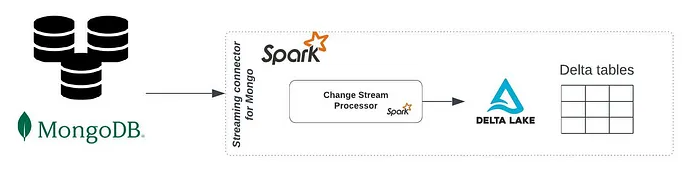
\includegraphics[scale=0.4]{images/data_transformation.png}}
\caption{Apache Spark Transforming Data in MongoDB Database}
\end{figure}
Repetitive transformations such as generating weekly reports can be hectic sometimes. As a remedy all the transformation will be automated using Airflow application.Batch processing pipelines are extremely useful in generating weekly/month/yearly sales reports, salary reports etc.\\[12pt]
\begin{figure}[H]
\centering
\fbox{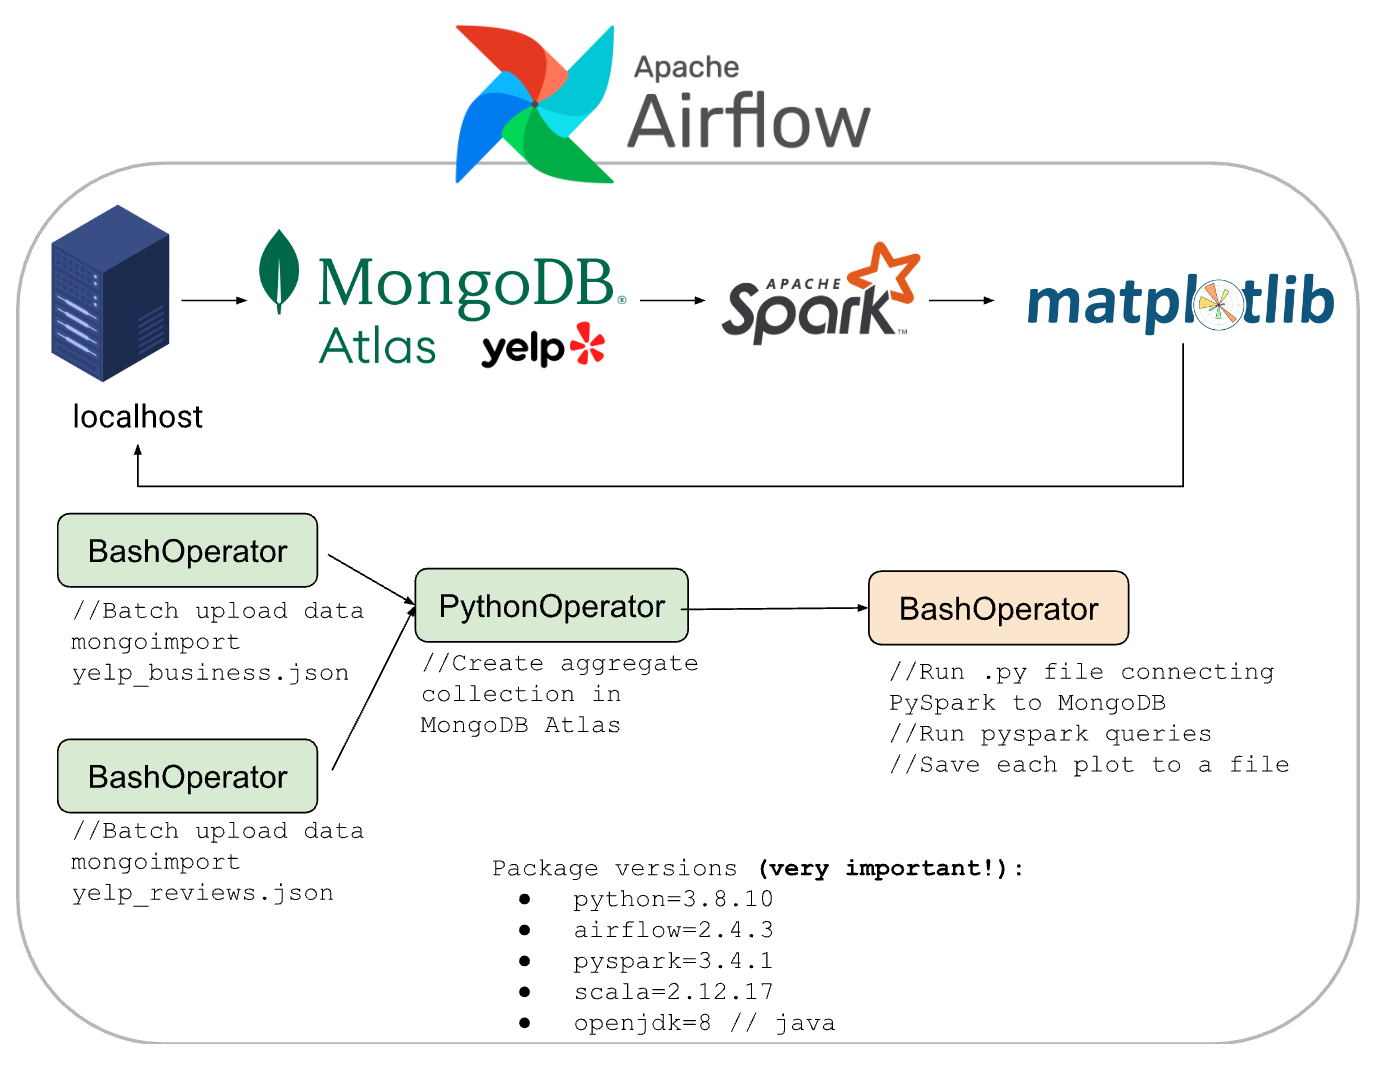
\includegraphics[scale=0.3]{images/automation.png}}
\caption{Apache AirFlow Automation}
\end{figure}
According to the golden rule of information, the value of data that is being generated stays constant for a certain period and the value of information starts to fade away with time. Robots in the production generate piles of data daily using sensors in real-time. These data may have a significant value. So, it would be unwise to ignore the data. Since the data experts are dealing with real-time data, they decided to deploy the stream processing method for the second pipeline. The ELT technique is used for the second pipeline due to the benefits offered. This pipeline has three phases too. The data produced by the robot sensors will be captured by the Apache Kafka software as events. Next the captured data will be stored in the MongoDB database in the loading phase. To transform the raw data to meaningful data, Apache Spark application will be used. In some case scenarios robots used to deviate from their normal operational task. The data migration timeline is divided into three stages: pilot phase, full rollout, and post migration optimization. A stream pipeline can solve this issue. As Apache Kafka extracts and stores data MongoDB database, Apache Spark will the raw data and detect for any anomalies in the real-time data. If the application detects an anomaly, it will alert the relevant IT professionals to the event. So that the IT professional could take the necessary steps to troubleshoot any issues in the robot or production line. The data migration timeline is divided into three stages, pilot phase, full rollout, and post migration optimization. In the pilot phase a small amount of data is migrated into MongoDB and tested. If the tested data is valid, all the data are migrated into the database in full rollout stage. Additional tinkering to the data is performed in the post migration optimization phase. Since Nexart have chosen MongoDB to store data, let us dig into the roots of MongoDB from the next section.
\chapter{MongoDB}
\section{History}
MongoDB database application is an application developed by Mongo Inc. This organization was founded by Dwight Merriman, Eliot Horowitz, and Kevin Ryan in 2007 \cite{Plugge2010-ie}. The first MongoDB application is introduced to the public as a platform between 2007 and 2008. Next Mongo Inc released their first NOSQL database in 2009. In 2017 MongoDB was listed in NASDAQ. MongoDB version 6 was released in 2022. The title of the application defines nature itself. The Humongous Ness of the application allows users to store a large quantity of data without worrying about the application's structure. MongoDB databases are used in IoT devices, mobile applications, real-time analysis, personalization, catalog management and content management. Enterprises such as Google, Facebook and Ebay deal with their growing data using MongoDB. Let us examine the marvel behind the MongoDB databases starting from the next chapter.
\section{Concepts}
The collections in MongoDB act as tables in relational databases while a document in a nonrelational database represents a row. A document has various fields labeled as columns in a relational database. Values are stored as key value pairs in MongoDB. Documents use the BSON format when storing values. The key features of MongoDB are aggregation, gridfs, sharding, document oriented, replication, schema less database, indexing, AD HOC Queries, and high performance \cite{noauthor_2018-nz}. MongoDB uses Data Modeling to store data. The relations between entities and the way the data is stored are defined as data modeling. It helps to build logical databases that are efficient. These databases offer low storage requirements, grant efficient data retrieval and limit redundancy. Through the data modeling process, the following objectives are archived.
\begin{itemize}
\item High Data Quality
\item Comprehension of dataflow and characteristics
\item Development and Maintenance
\item Performance
\end{itemize}
Data models are categorized into three types based on specificity/detail and they are conceptual, logical, and physical data models. One to One, one to many and Many to Many are relationship types that are used in data models. Embedded and Reference data models are two methods used for creating a model. Logical or mathematical operations are executed in MongoDB by using query operators. Query and projection, update and aggregation pipeline operators are examples for query operators.\\[12pt]
Regular expressions in NOSQL queries are used to match patterns in a document. List given below points out reasons for using regular expressions.
\begin{itemize}
\item Match text and define search patterns in sequences of characters. 
\item Retrieve data of an undefined field. 
\item Locate small subsets of data within a collection.
\end{itemize}
The database administrators can view only the necessary data in a document using the projection feature of MongoDB. Projection features come in handy when removing unnecessary fields from query results, retrieving indexed query results without fetching full documents and filtering data without causing any database performance issues. The sorting method in MongoDB defines the order in which query returns the matching documents in collection. The number of documents retrieved can be limited by using the limit method. Indexes in MongoDB aid in query data in an efficient manner. Avoidance of collection scans, effectiveness of indexing strategies and searching efficiency are achieved through the indexing mechanism. Single field, compound and multi key index are examples of indexes. Creation of a single index in a document is done by using single field index while references to multiple fields in a document is obtained through compound index. The values stored in arrays are indexed by multi key indexes. The data retrieval speed is enhanced by the advanced indexing feature. Geospatial, text and hashed indexing are techniques used in advanced indexing. Geospatial coordinate data are handled by 2d indexes and 2d sphere indexes. Text search queries are powered by text indexes. Entries with hashes are indexed using hash indexes. Gaining accurate results through processing multiple documents by selecting data from a collection is defined as aggregation \cite{noauthor_undated-pn}. Aggregation in MongoDB is performed using groups by clause and complex aggregation operations. It is performed to group values of multiple documents together and to fetch nested data to perform complex operations. In addition, it is used to filter and sort documents and analyze the changes in data. Match, group, sort and project are aggregation pipeline stages. Operations in aggregation are sum, average, minimum, maximum and push. Replication is the process of cloning the same data across multiple MongoDB servers. The intentions behind replication are listed below.
\begin{itemize}
\item Data redundancy and high availability. 
\item Making copies of data across servers. 
\item Performing data backups and recoveries. 
\end{itemize}
Replication is performed to increase the availability of data and to dampen the effects of a single server loss. MongoDB manages replication through replica sets. Collection of MongoDB nodes are defined as MongoDB nodes. At least three MongoDB nodes are required to form a replica set. All the writing operations are performed by the primary node while secondary nodes that are under the root node copy data from the primary node. When a primary node fails, it will be elected as a secondary node. The benefits and drawbacks of replication are discussed in the table given below.
\begin{table}[H]
\centering
\begin{tabularx}{\textwidth}{XX}\hline
Advantages & Disadvantages\\\hline
Availability & Higher usage of storage and network bandwidth.\\
Scalability & Higher levels of complexity in operation, configuration, and monitoring.\\
Enhanced Performance & Lags in propagation.\\
Disaster Recovery & Challenges in maintenance.\\
Continuous Operations & Consistency Issues\\\hline
\end{tabularx}
\caption{Benefits and Drawbacks of Replication}
\end{table}
The list given below highlights the limitations of replication.
\begin{itemize}
\item Difficulties in handling data and query traffic.
\item Inability of MongoDB instances to manage write operations. 
\item Inability to outsize memory regarding large datasets.
\item Higher costs.
\end{itemize}
The distribution process of data in MongoDB is designated as Sharding. A single dataset is stored in multiple databases. Sharding process adds more memory and processing units or ram into a single server. Sharding is associated with two types of scaling methods, and they are vertical and horizontal scaling. Adding more resources to the server is defined as vertical scaling while horizontal declares of adding more processing units or physical machines to the server or database. Sharding uses an architecture, and this architecture uses sharding clusters. A sharding cluster is formed out of multiple shards, mongos processes and configuration servers. Shard key distributes data among the shards and a shard key is automatically created by the database. The sharding process creates a cluster. A cluster of MongoDB instances forms at least three servers. The list below addresses the pros of sharding.
\begin{itemize}
\item Increased storage capacity.
\item Increased read/write throughput.
\item High availability.
\item Facilitates horizontal scaling.
\end{itemize}
The way multiple documents are logically connected to each other in MongoDB is represented in relationships. Database structures are refined by creating relationships between documents. In addition, they link up the entities in a database and make execution times shorter. Relationships in documents are categorized into embedded and reference relationships. Reference relationships are achieved through many to many relationships while embedded relationships are achieved through one to one and one to many relationships. Files that are greater than 16MB are stored using GridFS driver in MongoDB. GridFS mechanism divides large files into smaller chunks and stores them as separate documents. The list given below addresses the probable causes of using GridFS. 
\begin{itemize}
\item Giving the privilege of storing files that are greater than 16MB.
\item Giving the access to a portion of a file without loading the whole file.
\item Storing and syncing files and metadata across distributed systems.
\end{itemize}
By default, GridFS uses fs files and fs chunks to store the file’s metadata and the chunks. The data processing paradigm for condensing large volumes of data into useful aggregated results is defined as Map Reduce. This technique is mostly used for large datasets. Map, reduce and query functions are executed MapReduce method. Referencing documents stored in multiple collections or databases is performed by using the DBref option. Ref, ID, and DB parameters are used with the DBRef option. Cover queries use indexed fields to gain efficient results without searching a whole collection. Given below are scenarios when cover queries comes in handy.
\begin{itemize}
\item When all the fields in query are part of an index.
\item When all the fields returned in query are in the same index.
\item When there are no null values in fields.
\end{itemize}
All data which require an update is stored within a single document to maintain the atomicity. There are certain constraints regarding the atomicity of MongoDB, and they are listed below. 
\begin{itemize}
\item Zero support for multi document atomic transactions.
\item Only allows to perform atomic operations in a single document.
\item Atomocity is maintained and executed at the document level.
\end{itemize}
Set, inc, push, pull and rename are commands used in performing atomic operations. High throughput operations that insert retrieve and delete documents based on insertion order are stored as fixed collections under the capped collections. When collection size reaches over its maximum threshold, it starts to delete the old data autonomously. Due to the following reasons capped collections are used.
\begin{itemize}
\item To make sure that recently entered data stay in the database.
\item Automate the old data removal process.
\item Store cached data that needs regular refreshing.
\end{itemize}
Capped collections have their own characteristics, and they are listed below.
\begin{itemize}
\item Delete operations not allowed to be performed unless it is removed automatically.
\item All elements in a collection should have an equal size.
\item No indexing is required because of working queues.
\item Helps to maintain log files to troubleshoot any errors.
\end{itemize}
Mechanisms such as authorization and authentication safeguard the MongoDB database from unauthorized access. MongoDB gives the capability to data experts to create users, grant access control for the created users and authenticate users.\\[12pt]
Sectionizing a collection of related commands which should be executed with similar session options are defined as session commands. Examples for session commands are abortTransaction, commitTransaction, endSessions, killAllSessions, killAll SessionByPatterns, refreshSession, killSessions and startSession. Undoing modifications and restoring the database back to its normal condition is performed by abortTransaction command. The commitTransaction command saves the changes made by operations in a multi-document transaction before ending the transaction. Before terminating a session, the endSession command overrides the timeout window. Ongoing operations in a session are terminated by using the killSession command. Any sessions that are twined with declared patterns are terminated by the killSessionbyPattern command. MongoDB tools such as bsondump, mongodump, mongoexport, mongofiles, mongoimport, mongorestore, mongostat and mongotop help data engineers in the process of backing up and restoring the databases. MongoDB Atlas is a cloud-based data storage service. Management and monitoring of MongoDB deployments in enterprises are carried out by the MongoDB Ops Manager tool. MongoDB databases have pros and cons. They are discussed in the next section thoroughly.
\section{Advantages and Disadvantages}
The MongoDB inherits its benefits and drawbacks, and they are highlighted in the table below. 
\begin{table}[H]
\centering
\begin{tabularx}{\textwidth}{XX}\hline
Advantages & Disadvantages\\\hline
Open source & Issues related to consistency.\\
Easy to use & Consumes a lot of resources.\\
Highly flexible & Less capabilities in creating relations.\\
Advanced security features & Complexity of managing transactions.\\
High Availability & Less compatibility\\
Reliable Indexing & Maintenance and management\\
Flexible Schema &\\
High Performance &\\\hline
\end{tabularx}
\caption{Advantages and Disadvantages of MongoDB}
\end{table}
The next section discusses the application of MongoDB’s concepts towards the Nexart’s web application.
\chapter{MongoDB Application}
\section{Database}
We have already acknowledged the issue faced by the Nexart organization. To overcome the issue, the data engineers of Nexart changed the architecture of the database and they moved towards a non-relational database such as MongoDB. The data engineers understood they must make some alterations to meet the growing business' demands. So, they decided to migrate their data to MongoDB. The command given below creates a database in MongoDB database.
\begin{figure}[H]
\centering
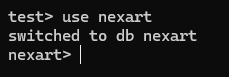
\includegraphics[scale=0.8]{images/database_creation_shell.png}
\caption{Nexart Database Creation}
\end{figure}
The creation of nexart database can be evaluated by executing the command given below. 
\begin{figure}[H]
\centering
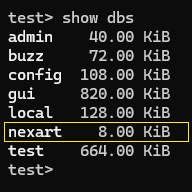
\includegraphics[scale=0.8]{images/database_creation_shell_confirmation.png}
\caption{Nexart Database Creation Confirmation}
\end{figure}
In prior to the migration, the database engineers map entities, and their attributes of the MSSQL database to MongoDB database. This process is discussed further in the collections section.
\section{Collections}
According to concepts of relational databases, all the entities are defined as tables. These tables were converted into collections in the MongoDB database. The tables in the MSSQL database inherited their own columns. These columns were mapped to the fields of the corresponding collections. Each table of the MSSQL database consists of 100 records each. These records are mapped to documents in MongoDB database. According to this scenario clients, branches, products, orders, and stock requests represent tables in relational databases while they are declared as collections in non-relational databases. The figure given below demonstrates the commands that should be executed to create the mentioned collections above. 
\begin{figure}[H]
\centering
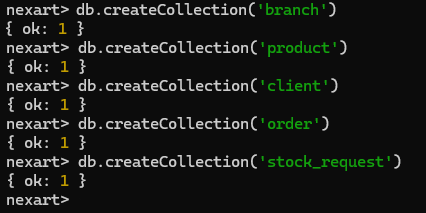
\includegraphics[scale=0.8]{images/collection_creation_shell.png}
\caption{Shell Collection Creation}
\end{figure}
The created collections can be verified by executing the command given below.
\begin{figure}[H]
\centering
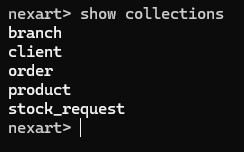
\includegraphics[scale=0.8]{images/collection_creation_shell_confirmation.png}
\caption{Collection Creation Verification}
\end{figure}
The next segment discusses the application of Mongo Shell regarding the development of Nexart’s web application. 
\section{Mongo Shell}
Before migrating data into the database, a database and tables should be created. While creating the tables primary keys, foreign keys and composite primary keys should be defined. So that it enables us to map the relations between the entities. The database administrators in the past used a command line interface to interact with the application. This applies to the database management systems in the past as well. Before the graphical user interface of MSSQL became known, the administrators used MSSQL cmd to create databases, tables etc. The Shell of MongoDB performs the same role as the CMD of MSSQL. When creating tables, they were required to provide a structure for the tables. Since MongoDB handles semi-structured and unstructured data well, there is no need to define the table structure. Even though the database, collections and column names should be named properly. So that it would help the software developers of the IT department to populate the data of the database in the Nexart web application. Queries are inserted and executed in Mongo Shell to perform all the database operations. As the collection creation phase is completed, the migration process remains. Data experts of Nexart exported the records in the MSSQL database to json files. The list below shows the data extracted from the tables.
\begin{itemize}
\item clients.json
\begin{figure}[H]
\centering
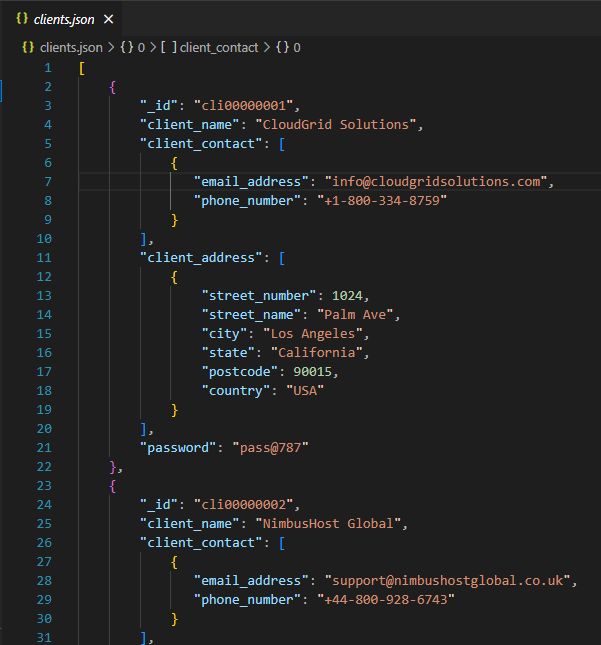
\includegraphics[scale=0.4]{images/clients_json.png}
\caption{Client JSON File}
\end{figure}
\item branches.json
\begin{figure}[H]
\centering
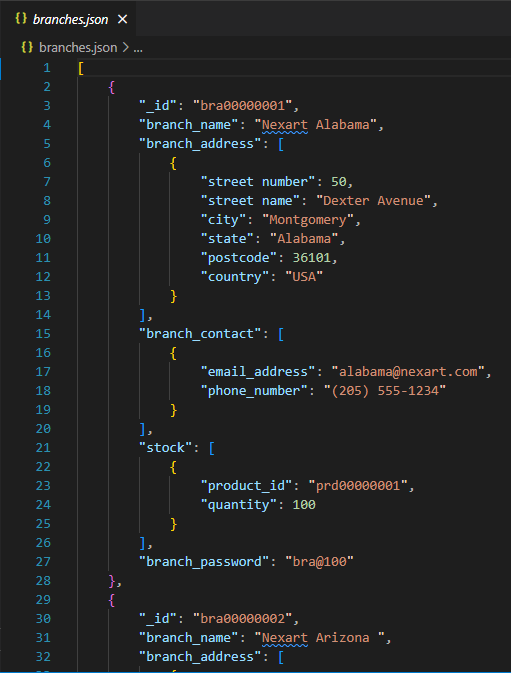
\includegraphics[scale=0.4]{images/branches_json.png}
\caption{Branches JSON File}
\end{figure}
\item products.json
\begin{figure}[H]
\centering
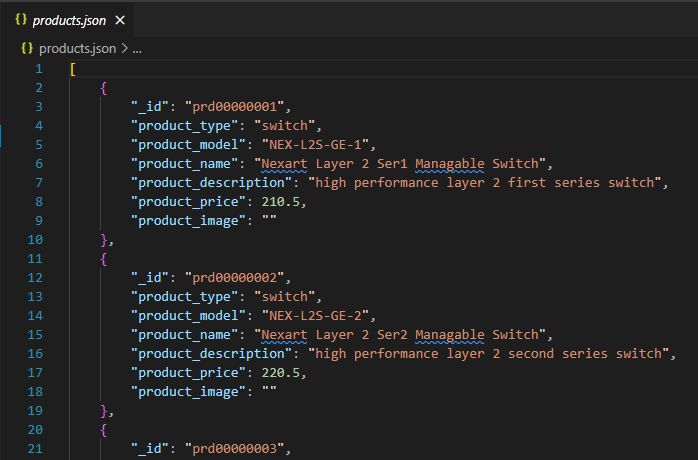
\includegraphics[scale=0.4]{images/products_json.png}
\caption{Products JSON File}
\end{figure}
\item orders.json
\begin{figure}[H]
\centering
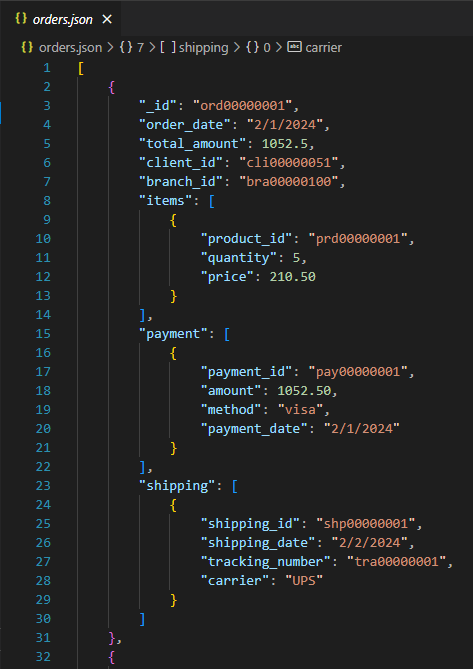
\includegraphics[scale=0.4]{images/orders_json.png}
\caption{Orders JSON File}
\end{figure}
\item stock requests.json
\begin{figure}[H]
\centering
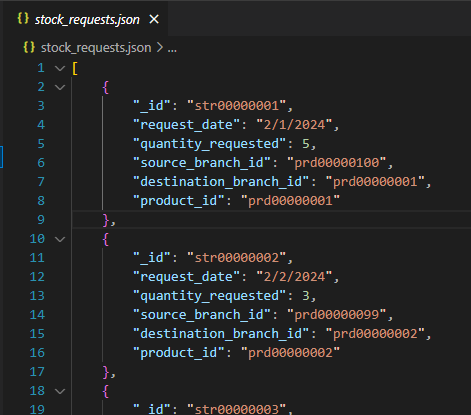
\includegraphics[scale=0.4]{images/stock_request_json.png}
\caption{Stock Requests JSON File}
\end{figure}
\end{itemize}
Since the MongoDB documents are represented in BSON format, MongoDB is compatible with handling json files as well. In the next phase all json files are imported into the relevant collections of the Nexart database in MongoDB server using mongoimport tool. The progress of the data imports is given below. 
\begin{itemize}
\item Client collection data import
\begin{figure}[H]
\centering
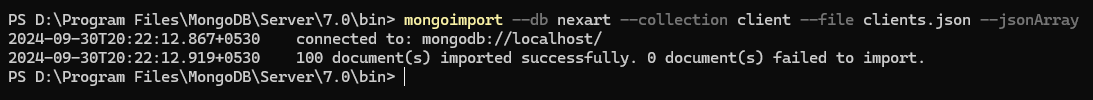
\includegraphics[scale=0.5]{images/client_data_import.png}
\caption{Client Collection Data Import}
\end{figure}
\item Branch collection data import
\begin{figure}[H]
\centering
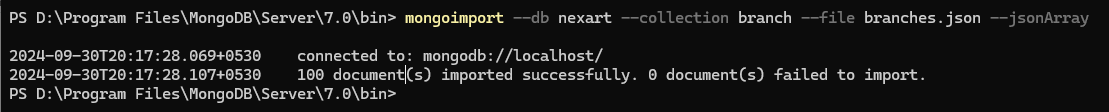
\includegraphics[scale=0.5]{images/branch_data_import.png}
\caption{Branch Collection Data Import}
\end{figure}
\item Product collection data import
\begin{figure}[H]
\centering
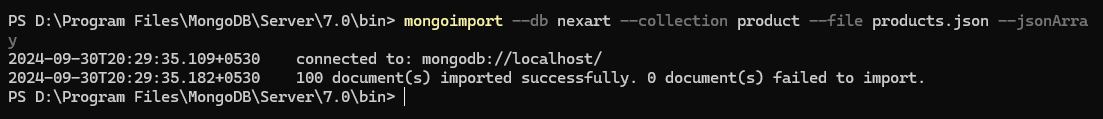
\includegraphics[scale=0.5]{images/product_data_import.png}
\caption{Product Collection Data Import}
\end{figure}
\item Order collection data import
\begin{figure}[H]
\centering
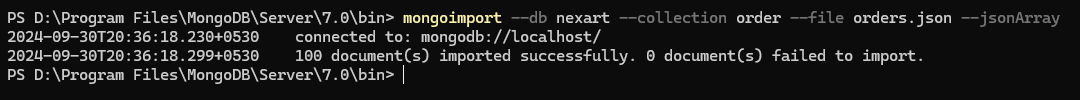
\includegraphics[scale=0.5]{images/order_data_import.png}
\caption{Order Collection Data Import}
\end{figure}
\item Stock Request data import
\begin{figure}[H]
\centering
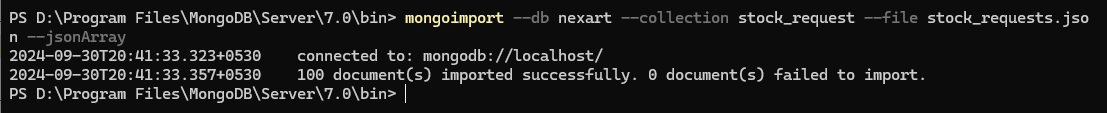
\includegraphics[scale=0.5]{images/stock_request_data_import.png}
\caption{Stock Request Collection Data Import}
\end{figure}
\end{itemize}
Next the data engineers wanted to make sure wither the data is imported into the relevant collections. By executing the commands given below they verified the import process of each collection.
\begin{itemize}
\item Clients
\begin{figure}[H]
\centering
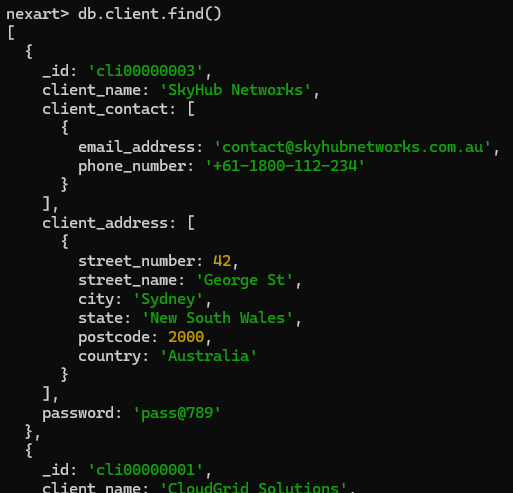
\includegraphics[scale=0.5]{images/client_data_import_confirmation.png}
\caption{Client Data Import Confirmation}
\end{figure}
\item Branches
\begin{figure}[H]
\centering
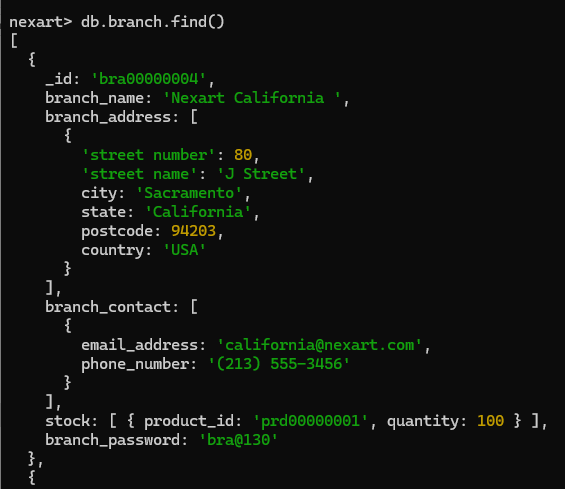
\includegraphics[scale=0.4]{images/branch_data_import_confirmation.png}
\caption{Branch Data Import Confirmation}
\end{figure}
\item Products
\begin{figure}[H]
\centering
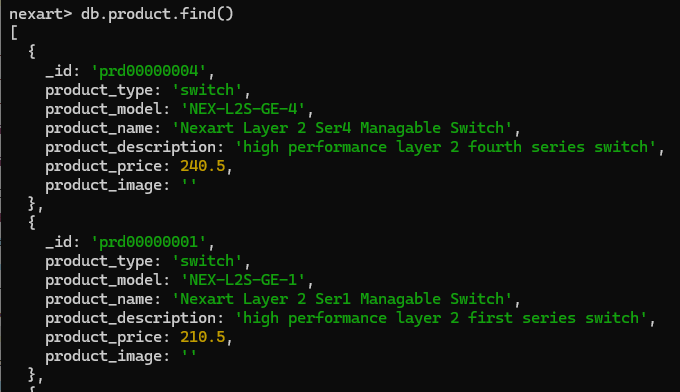
\includegraphics[scale=0.4]{images/product_data_import_confirmation.png}
\caption{Product Data Import Confirmation}
\end{figure}
\item Orders
\begin{figure}[H]
\centering
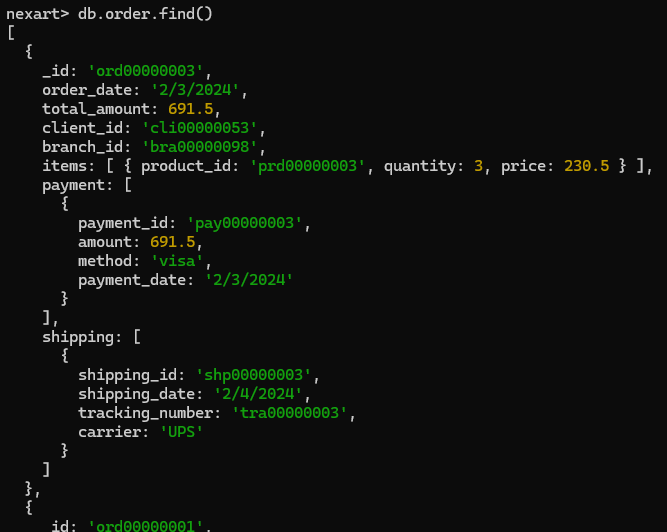
\includegraphics[scale=0.4]{images/order_data_import_confirmation.png}
\caption{Order Data Import Confirmation}
\end{figure}
\item Stock Requests
\begin{figure}[H]
\centering
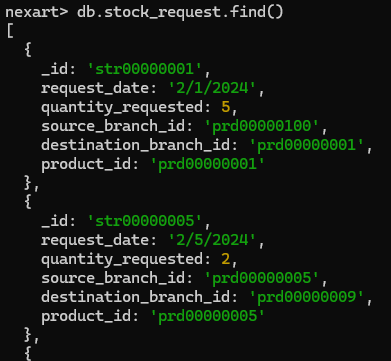
\includegraphics[scale=0.4]{images/stock_request_data_import_confirmation.png}
\caption{Stock Request Data Import Confirmation}
\end{figure}
\end{itemize}
Hence the records displayed at screen are limited to 20 per each iteration, they get the document statics of each collection by executing the commands given below.
\begin{figure}[H]
\centering
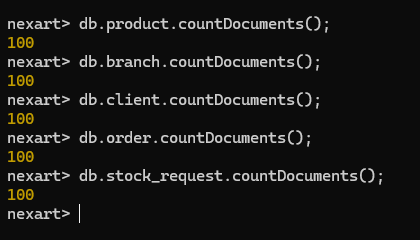
\includegraphics[scale=0.5]{images/collections_document_count.png}
\caption{Document Statistics of Collections}
\end{figure}
There are differences between the query structures of relational databases and non-relational databases. With the growth of data, the database queries got complex, and some admins were bored of typing the same query repeatedly. In addition, it took some time to insert the query and human errors such as typos occurred as well. In addition, only highly technical professionals of Nexart understood SQL/NOSQL while for other users of Nexart, did not comprehend SQL/NOSQL. So, the developers of MSSQL produced a solution to address these issues.
\section{Mongo Compass}
The previous chapter brought up an issue regarding the usability of MSSQL CMD/Mongo Shell. As a remedy for this issue, MSSQL developed a graphical user interface along with a CMD. This resulted in fewer errors and query response times were improved. Even if the query is entered correctly, an admin can mistake enter a wrong value in the field and make the data inefficient. So, the admin is solely responsible for the validity of data. MongoDB Compass functions similarly as MSSQL GUI. As a result of the development of Mongo Compass, technical people who have an average knowledge about databases of Nexart do not need to worry about entering data into the database. The image given below depicts the viewing of the created Nexart database.
\begin{figure}[H]
\centering
\fbox{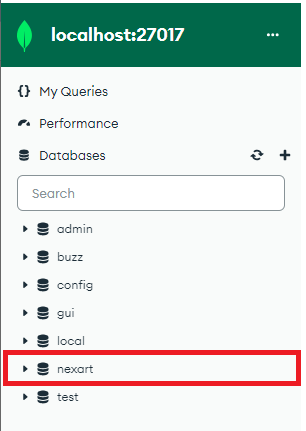
\includegraphics[scale=0.5]{images/database_creation_compass_confirmation.png}}
\caption{Nexart Database Creation Mongo Compass Confirmation}
\end{figure}
Earlier branch, client, product, order, and stock request collections were created in the Nexart database. The image below shows the created collections visually in Mongo Compass.
\begin{figure}[H]
\centering
\fbox{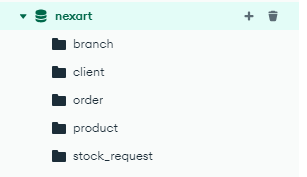
\includegraphics[scale=0.5]{images/collection_creation_compass confirmation.png}}
\caption{Created Collections Visual Confirmation}
\end{figure}
The data engineers imported data into the collections. All imported data can be verified visually by the list given below.
\begin{itemize}
\item Branch Collection
\begin{figure}[H]
\centering
\fbox{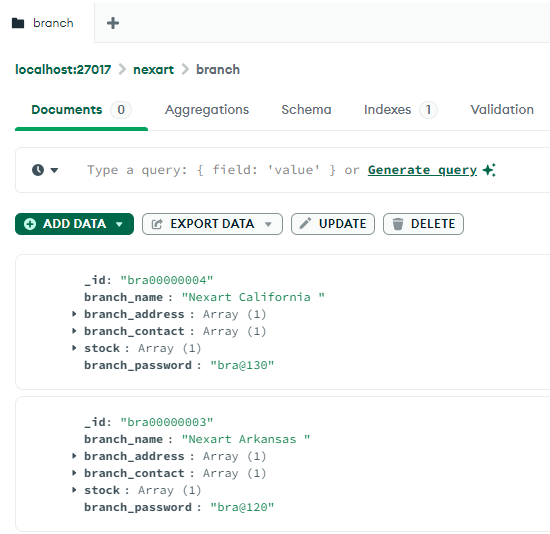
\includegraphics[scale=0.4]{images/branch_compass.png}}
\caption{Branch Imported Data Visual Confirmation}
\end{figure}
\item Client Collection
\begin{figure}[H]
\centering
\fbox{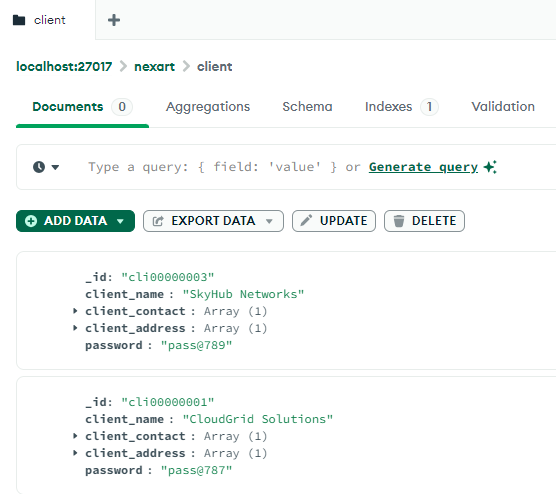
\includegraphics[scale=0.4]{images/client_compass.png}}
\caption{Client Imported Data Visual Confirmation}
\end{figure}
\item Product Collection
\begin{figure}[H]
\centering
\fbox{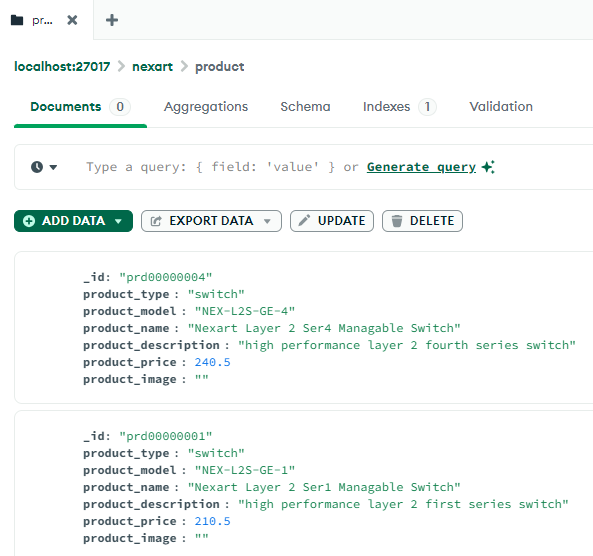
\includegraphics[scale=0.4]{images/product_compass.png}}
\caption{Product Imported Data Visual Confirmation}
\end{figure}
\item Order Collection
\begin{figure}[H]
\centering
\fbox{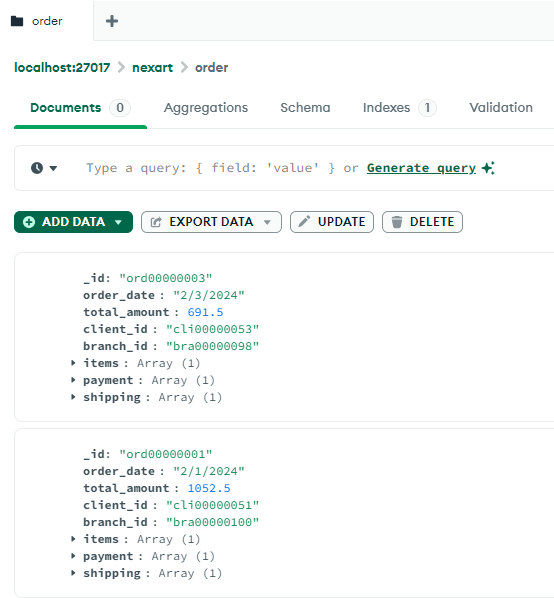
\includegraphics[scale=0.4]{images/order_compass.png}}
\caption{Order Imported Data Visual Confirmation}
\end{figure}
\item Stock Request Collection
\begin{figure}[H]
\centering
\fbox{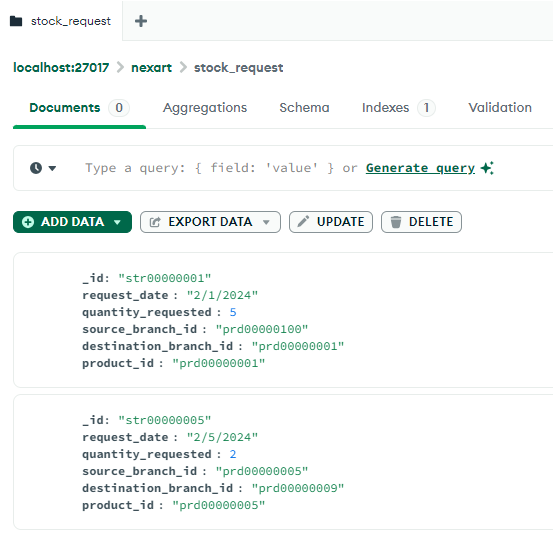
\includegraphics[scale=0.4]{images/stock_request_compass.png}}
\caption{Stock Request Imported Data Visual Confirmation}
\end{figure}
\end{itemize}
People with average technical knowledge can enter data into the database via MongoDB compass’s user-friendly graphical interface. Even though this graphical user interface had a limitation, it is addressed in the next chapter.
\chapter{Development of MongoDB Application}
\section{Technical Stack and Environment Setup}
Sometimes graphics are not enough to convey a message. The message should be to understand the users. This applies to the web applications as well. An application contains two parts, and they are front-end and back-end. All the users deal with the front-end of the application while all the processes occur in the back-end of the application. Since the developers of Nexart are familiar with Node JS, Express JS, HTML, CSS, Bootstrap, JavaScript and MongoDB, the development team decided to use the same technical stack to develop the Nexart’s web application.
\begin{figure}[H]
\centering
\fbox{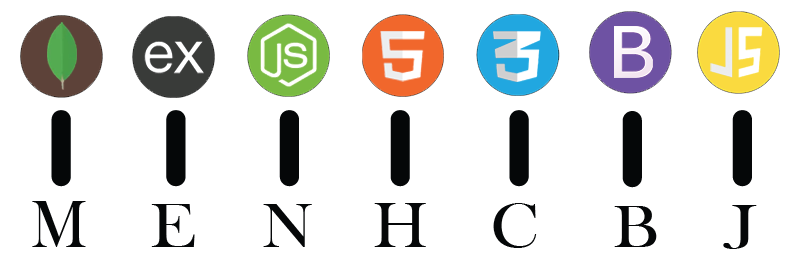
\includegraphics[scale=0.4]{images/technical_stack_1.png}}
\caption{Technical Stack}
\end{figure}
\begin{itemize}
\item M - MongoDB
\item E - Express JS
\item N - Node JS
\item H - HTML
\item C - CSS
\item B - Bootstrap
\item J - JavaScript
\end{itemize}
Before jumping into the front development, the development environment should be organized. Many developers of Nexart prefer Visual Studio Code IDE over other IDEs due to support offered by the vs community. So, all the developers agreed to go with Visual Studio Code.
\begin{figure}[H]
\centering
\fbox{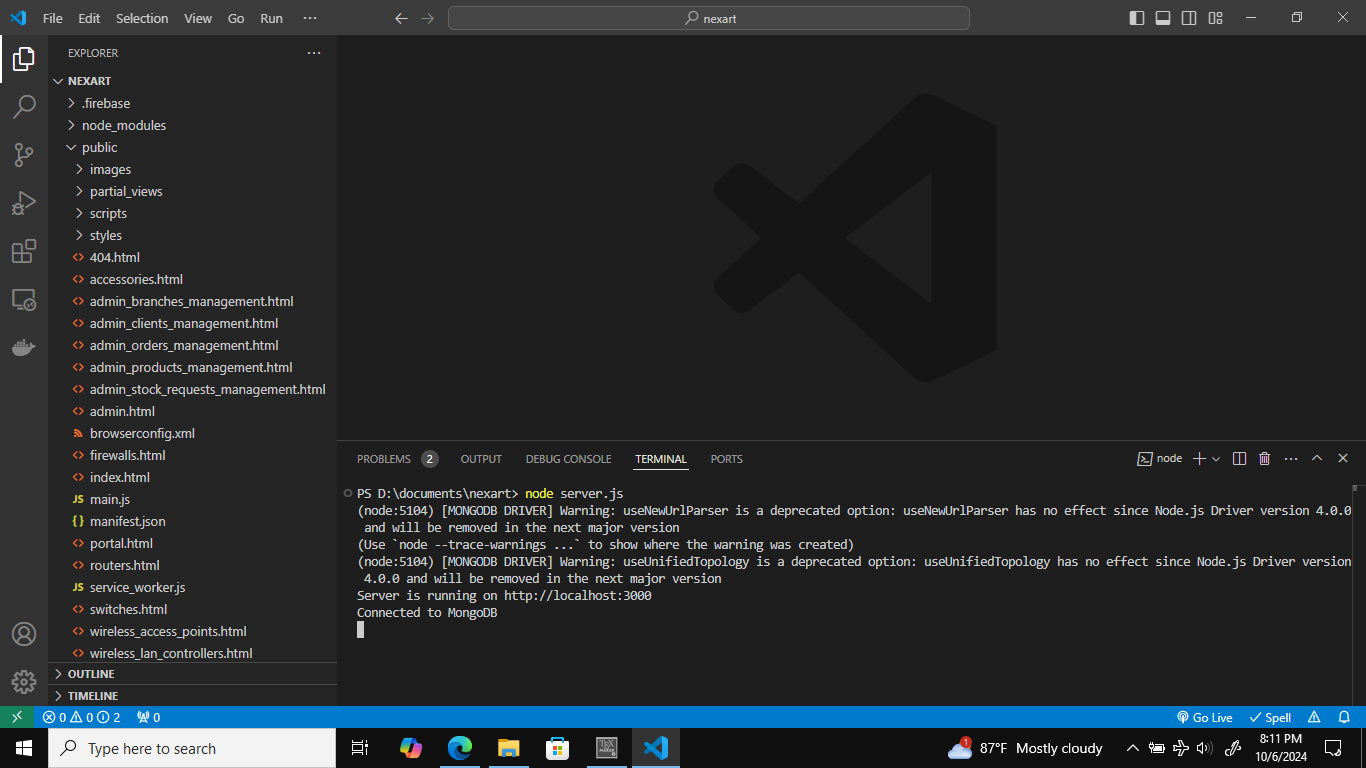
\includegraphics[scale=0.3]{images/IDE.png}}
\caption{Integrated Development Environment}
\end{figure}
Housekeeping is a main aspect in application development. This makes sure that every is organized. In addition, it makes error troubleshooting easier. The Nexart web application’s file structure is given below.
\begin{figure}[H]
\centering
\fbox{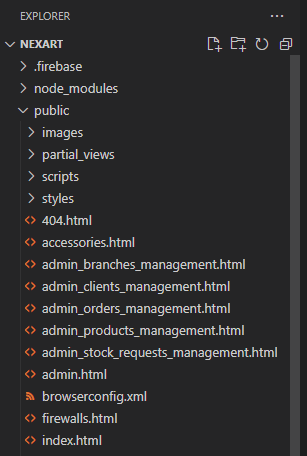
\includegraphics[scale=0.5]{images/application_file_structure.png}}
\caption{Project File Structure}
\end{figure}
As the technical stack and environment have already been organized, the front-end development of the application commenced from the next chapter onwards.
\section{Front-end Development}
Before discussing the font-end of the application, let us get to know about the technical users in society. We can categorize technical people into 3 categories, and they are listed below.
\begin{itemize}
\item People who have less technical knowledge.
\item People who have average technical knowledge.
\item People who have high technical knowledge.
\end{itemize}
Let us explore facts about each technical group. People with less technical people are digitally literate people who use digital devices such as smart phones to complete some their daily/non-daily activities such as browsing the web, streaming music/videos online, replying to emails etc. Average technical personnels have more technical knowledge in comparison to people with less technical knowledge. They are also digitally literate who perform tasks such as word processing, spreadsheet processing, slide processing, using simple database management systems such as Microsoft Office Access etc. Highly technical people are digitally literate as averagely technical people, but they perform advanced tasks such as software development, writing SQL/NOSQL queries to manipulate data, writing scripts to automate tasks etc. So highly technical people are capable of handling command line interfaces and graphical user interfaces of database management systems while averagely technical users capable of only handling graphical user interfaces of databases. People with less technical capabilities are not capable of handling either command line interfaces or graphical user interfaces of databases.\\[12pt]
This applies to the Nexart enterprise as well. Nexart web application can be accessed by the user categorizes that are mentioned in the above paragraph. As for instance circuit programmers, administrators and floor staff represents highly technical, averagely technical, and less technical people accordingly. In some cases, people who have less technical capabilities need to store data in the database to process a task such as monthly payroll. So, they need to interact with MongoDB database indirectly to process the payroll. This is where the font-end of the web application comes into play. This gives the privilege to the less technical people to interact with the database. Before developing the front-end wireframes were sketched out and they are demonstrated below.
\begin{itemize}
\item Admin Product Management Wireframe
\begin{figure}[H]
\centering
\fbox{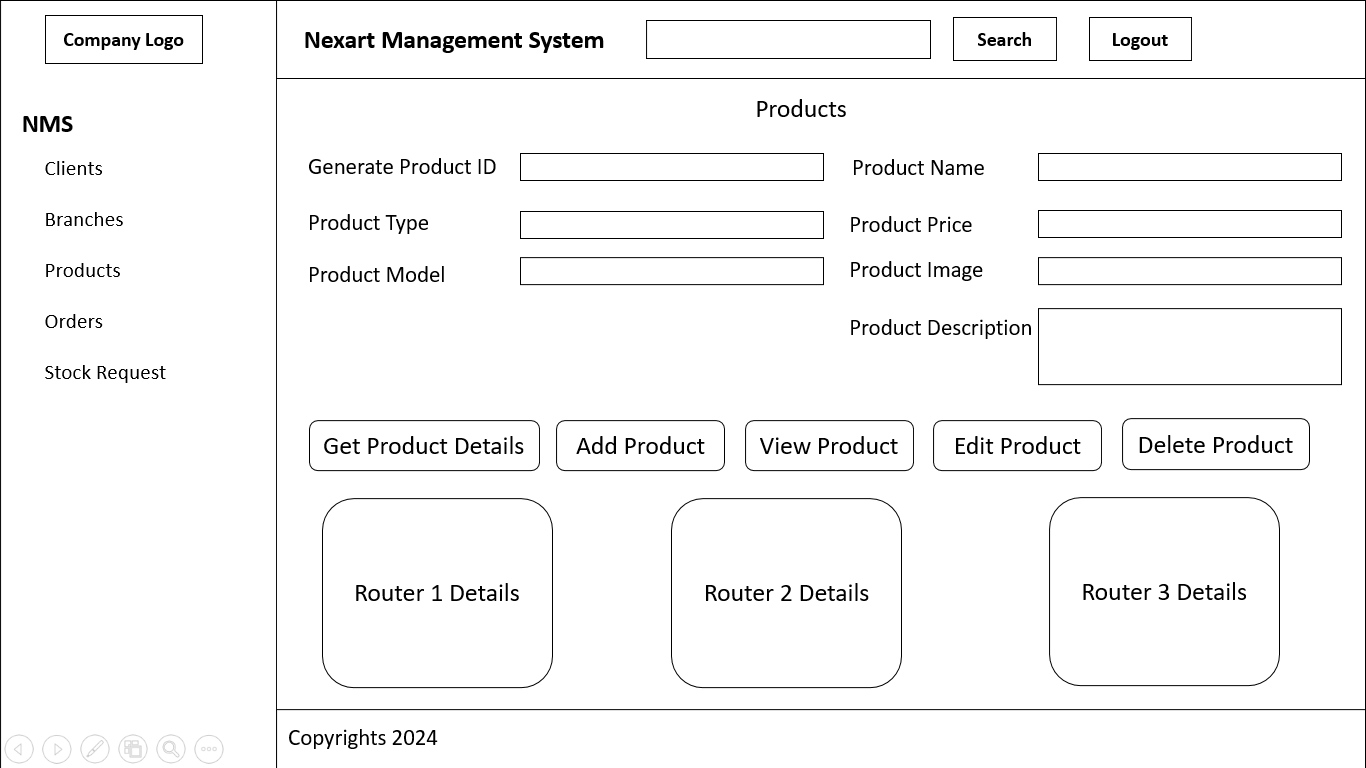
\includegraphics[scale=0.3]{images/admin_product_management_wireframe.png}}
\caption{Admin Product Management Wireframe}
\end{figure}
\item Routers Wireframe
\begin{figure}[H]
\centering
\fbox{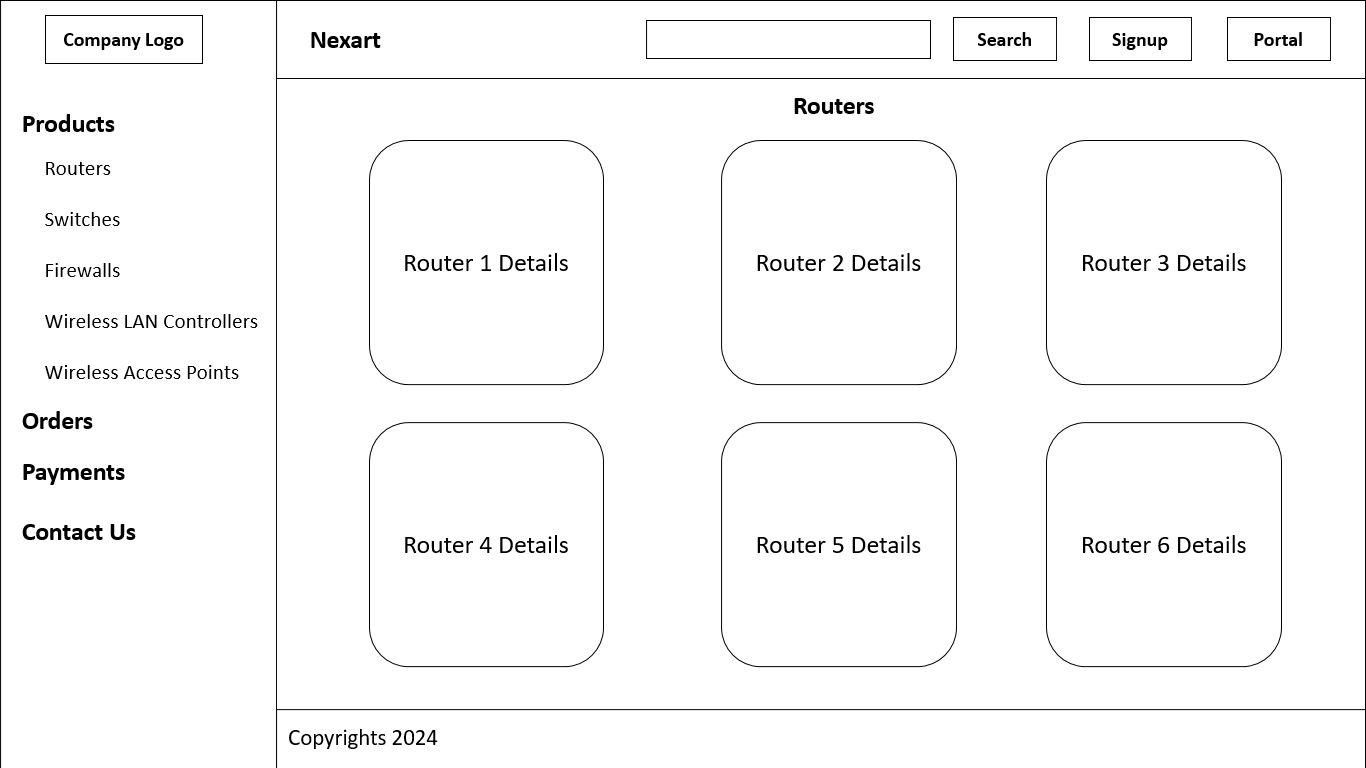
\includegraphics[scale=0.3]{images/routers_wireframe.png}}
\caption{Routers Wireframe}
\end{figure}
\item Switches Wireframe
\begin{figure}[H]
\centering
\fbox{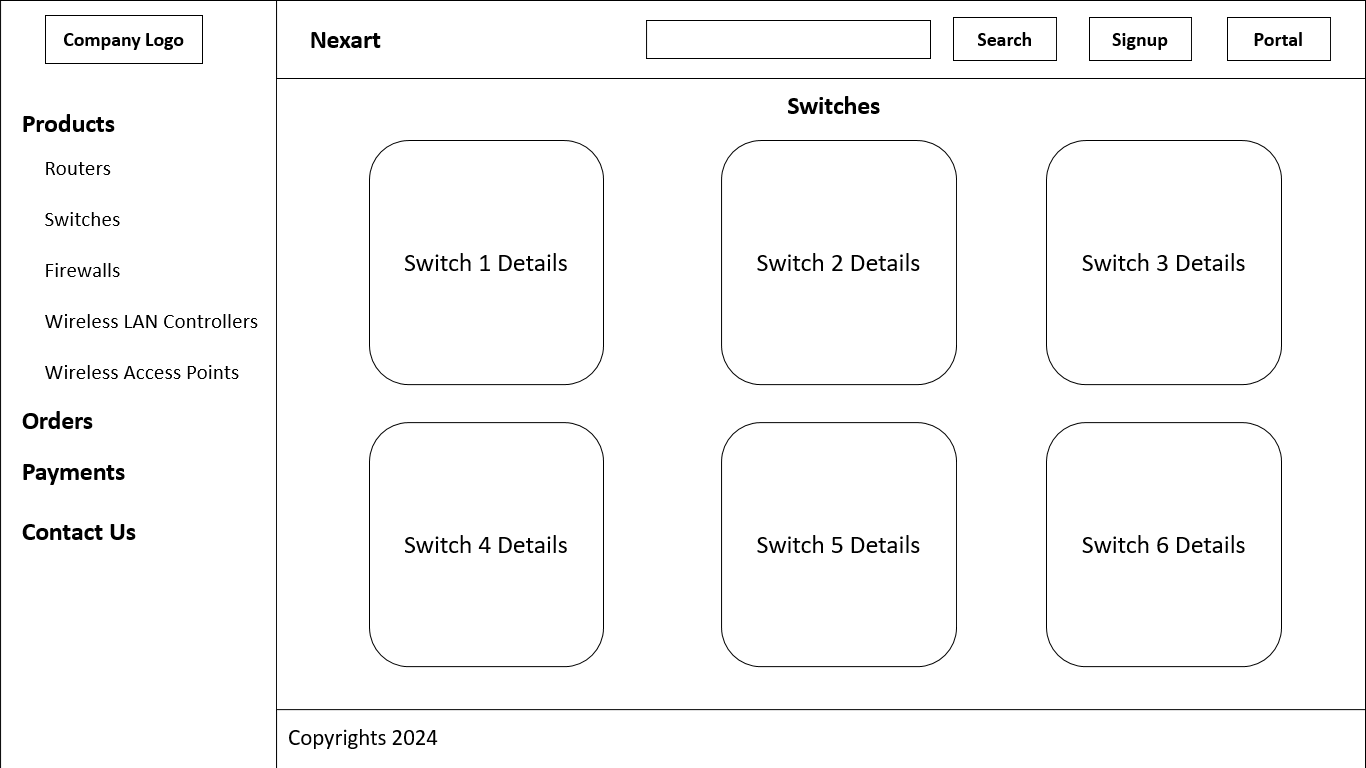
\includegraphics[scale=0.3]{images/switches_wireframe.png}}
\caption{Switches Wireframe}
\end{figure}
\item Firewalls Wireframe
\begin{figure}[H]
\centering
\fbox{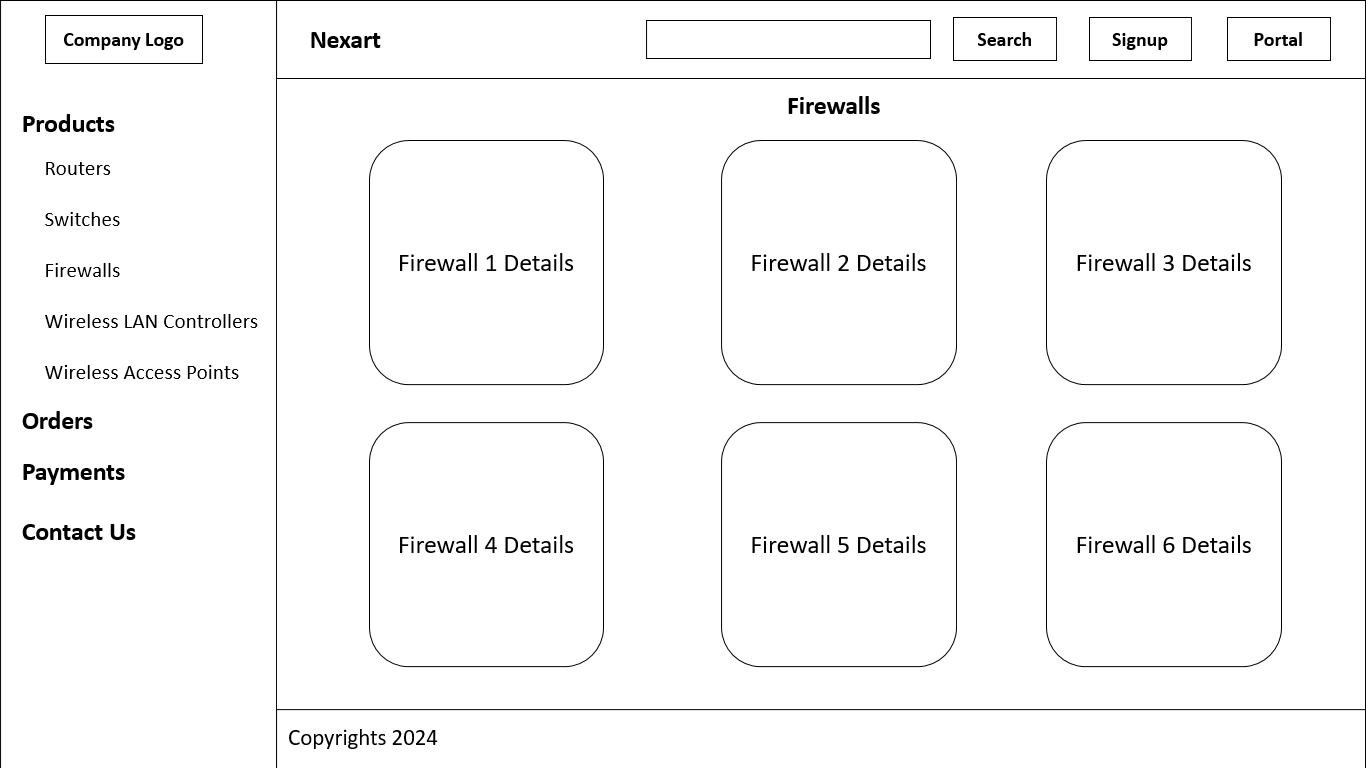
\includegraphics[scale=0.3]{images/firewalls_wireframe.png}}
\caption{Firewalls Wireframe}
\end{figure}
\end{itemize}
In the next chapter these wireframes are brought back to life. 
\subsection{Graphical User Interface}
In order develop the graphical user interfaces html and bootstrap technologies are used and the developed graphical user interface illustrated below.\\[12pt]
\begin{itemize}
\item Index Page
\begin{figure}[H]
\centering
\fbox{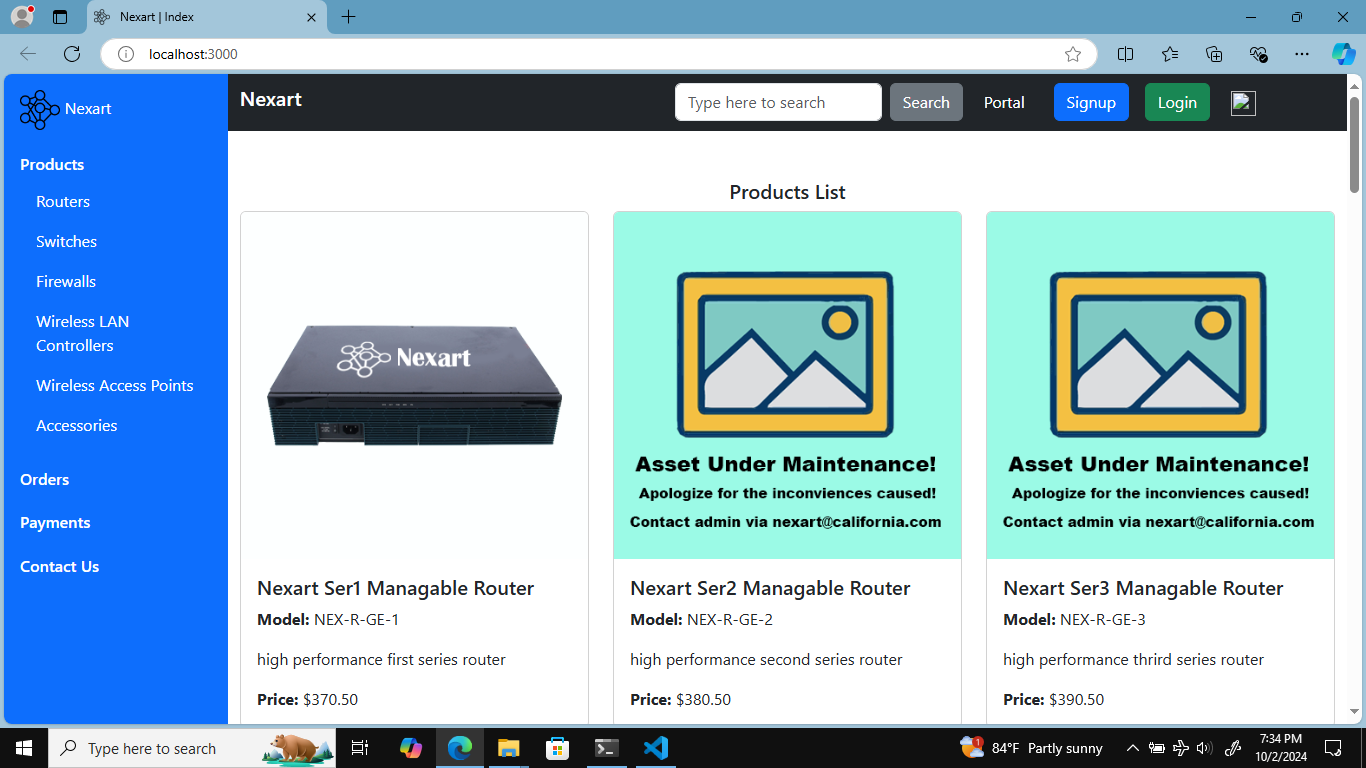
\includegraphics[scale=0.3]{images/index_page.png}}
\caption{Index Page}
\end{figure}
\item Product Management Page
\begin{figure}[H]
\centering
\fbox{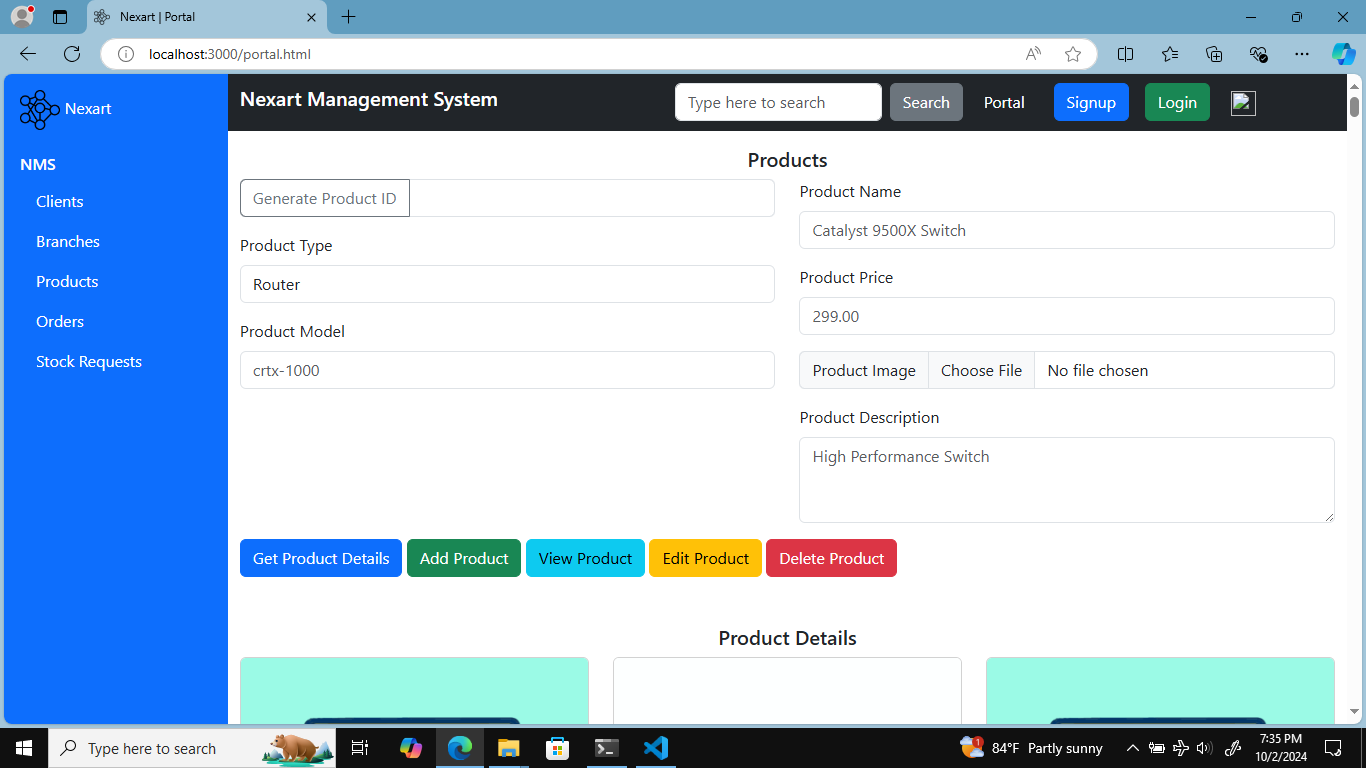
\includegraphics[scale=0.3]{images/product_management.png}}
\caption{Product Management Page}
\end{figure}
\item Routers Page
\begin{figure}[H]
\centering
\fbox{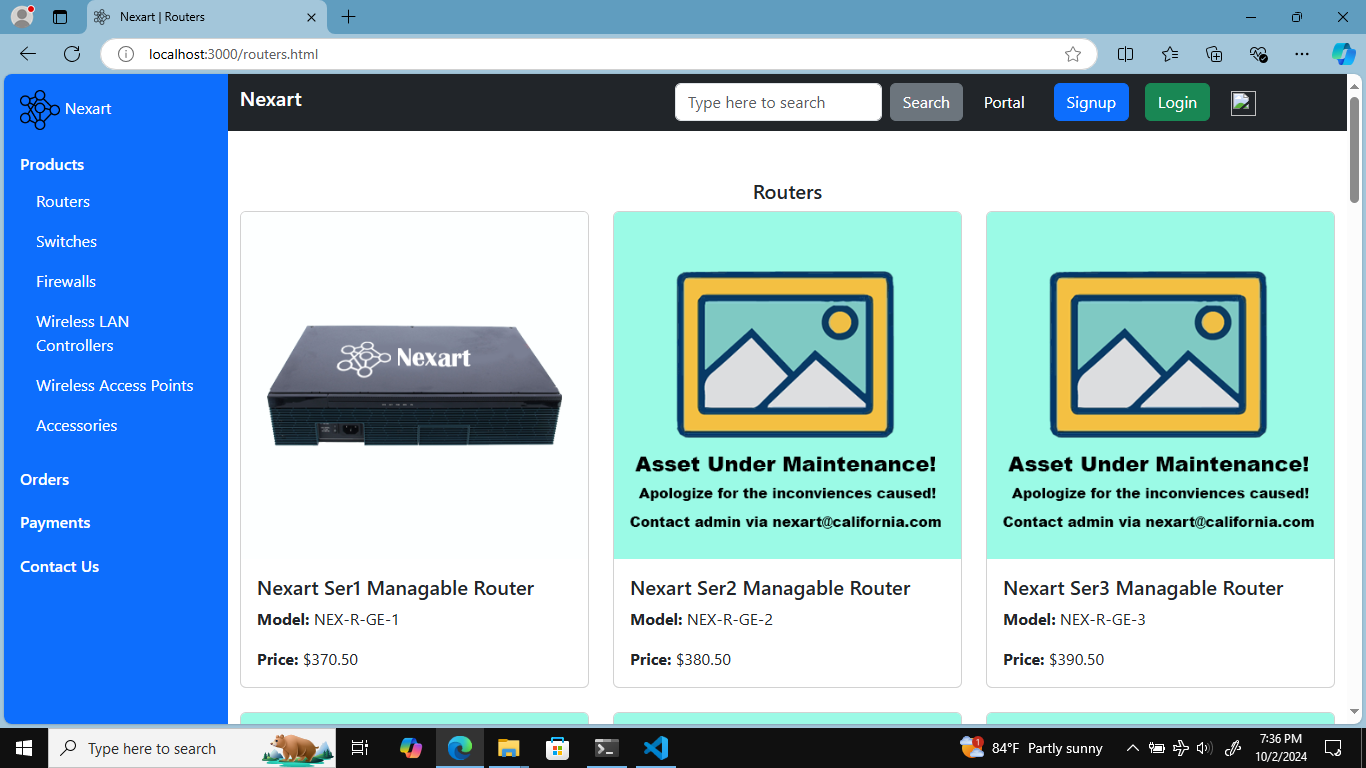
\includegraphics[scale=0.3]{images/routers_page.png}}
\caption{Routers Page}
\end{figure}
\item Switches Page
\begin{figure}[H]
\centering
\fbox{\includegraphics[scale=0.3]{images/switches_page.png}}
\caption{Switches Page}
\end{figure}
\item Firewall Page
\begin{figure}[H]
\centering
\fbox{\includegraphics[scale=0.3]{images/firewalls_page.png}}
\caption{Firewalls Page}
\end{figure}
\item Wireless LAN Controller Page
\begin{figure}[H]
\centering
\fbox{\includegraphics[scale=0.3]{images/wireless_lan_controller_page.png}}
\caption{Wireless LAN Controllers Page}
\end{figure}
\item Wireless Access Point Page
\begin{figure}[H]
\centering
\fbox{\includegraphics[scale=0.3]{images/wireless_access_point_page.png}}
\caption{Wireless Access Points Page}
\end{figure}
\item Accessories Page
\begin{figure}[H]
\centering
\fbox{\includegraphics[scale=0.3]{images/accessories_page.png}}
\caption{Accessories Page}
\end{figure}
\end{itemize}
Graphical User Interfaces does not complete the whole development phase of the application. Front-end of the application needs to communicate with the databases to perform all crud operations. Back-end of the application connects the front-end to the database. The next segment chapter discusses the development of back-end.
\section{Back-end Development}
The back-end of the application is developed using JavaScript. Scripts that are related to back-end are shown below.
\begin{itemize}
\item Server JS
\begin{figure}[H]
\centering
\includegraphics[scale=0.5]{images/server_js_backend.png}
\caption{Server JS Backend}
\end{figure}
\item Admin Product Management
\begin{figure}[H]
\centering
\includegraphics[scale=0.5]{images/admin_product_management_backend.png}
\caption{Admin Product Management Backend}
\end{figure}
\end{itemize}
The server JavaScript file is the main script of this application. Functionality of the scripts of webpages relies upon the server JavaScript file. In this manner backend development comes into a whole. The functionality of the system is evaluated in the next chapter.
\section{Testing}
Without system testing and bug fixing, the whole development phase is not complete. The application cannot be hosted online unless the testing phase is completed. So, the development team requested the quality assurance engineer to evaluate the system thoroughly. For starters he tested the crud functionality of the products in the application by inserting values and triggering events such as clicks in admin product management page. The results of the crud functionality are given below.
\begin{table}[H]
\centering
\begin{tabularx}{\textwidth}{XXXXXXXX}\hline
Test Case ID & Description & Precondition & Test Procedure & Test Inputs & Expected Output & Actual Output & Results\\\hline
TC0001 & Admin adding a product into the database. & Admin should be logged in and system should be up and running. & Filling up the input fields and click on add product button & product id, product name & Product added successfully & Product added successfully & \fbox{\includegraphics[scale=0.3]{images/product_added_confirmation.png}}\\
TC0002 & Admin viewing a product. & Admin should be logged in and system should be up and running. & Insert product id in and click on view product button & product id & Product fetched! & Product fetched! & \fbox{\includegraphics[scale=0.3]{images/product_fetched_confirmation.png}}\\
TC0003 & Admin editing a product. & Admin should be logged in and system should be up and running. & Fill up the necessary fields and click on edit product button & product id, product name & Product updated successfully! & Product updated successfully! & \fbox{\includegraphics[scale=0.3]{images/product_update_confirmation.png}}\\
TC0002 & Admin deleting a product. & Admin should be logged in and system should be up and running. & Insert product id in and click on remove product button & product id & Product deleted successfully! & Product deleted successfully! & \fbox{\includegraphics[scale=0.3]{images/product_delete_confirmation.png}}\\\hline
\end{tabularx}
\caption{CRUD Test Case Results}
\end{table}
In this manner the QA tested crud operations for other collections as well. In addition, he conducted unit and integration testing for all the scripts in the application. Since the testing phase has already been completed, the nexart web application is ready to be deployed online. Even though the system is fully developed, maintenance should be carried out to address the technical issues that are about to occur in the future. The effectiveness of the implemented data engineering pipeline is evaluated in the next segment.
\chapter{Data Analytics}
\section{Analytical Questions}
Values insights about the business can be drawn from the documents stored in the collections. According to the perspective of the business we can derive questions, and these questions are divided into several categories. The question categories and the relevant question for each category are listed below.
\begin{enumerate}
\item Orders and Client Behavior
	\begin{itemize}
	\item What is the most ordered product item across all branches?  
	\item Which product item have been ordered a lot in quantity wise?
	\item Which payment method is preferred by most of the clients? 
	\item Which branch has received the most orders? 
	\item What is the frequency of making repeat orders?  
	\end{itemize}
\item Stock and Inventory Management 
	\begin{itemize}
	\item Which branch receives the highest amount of stock requests? 
	\item How long does it take branch to receive a requested product?  
	\item What is the product item in stocks that has the highest quantity across all branches?  
	\item Which product items are low in quantity wise and have made the highest requests?  
	\item What is the relationship between stock requests and client orders?
	\end{itemize}
\item Branch and Operational Efficiency 
	\begin{itemize}
	\item Which branch generates the highest sales?  
	\item How long does it take for a product shipment to get delivered to the client?
	\item Which shipping carriers take the least amount of time to deliver products to clients?
	\item Which branch generates the least sales?
	\item What product prices are different branch wise and what is their impact on sales? 
	\end{itemize}
\item Client Satisfaction and Payment Analysis
	\begin{itemize}
	\item What is the correlation between the payment method and client order volume?
	\item What impact does the shipping cost and times of products have on client’s address?  
	\item Which branch gets the most complaints and returns?
	\item How do quicker deliveries affect client order amounts?
	\end{itemize}
\end{enumerate}
The questions mentioned in the above help us understand the status of the business. The answers to some queries are listed below.
\begin{itemize}
\item What is the most ordered product item across all branches?
\begin{figure}[H]
\centering
\includegraphics[scale=0.5]{images/Q1.1.png}
\caption{Question 1.1 Answer}
\end{figure}
\item Which product item have been ordered a lot in quantity wise?
\begin{figure}[H]
\centering
\includegraphics[scale=0.5]{images/Q1.2.png}
\caption{Question 1.2 Answer}
\end{figure}
\item Which payment method is preferred by most of the clients?
\begin{figure}[H]
\centering
\includegraphics[scale=0.5]{images/Q1.3.png}
\caption{Question 1.3 Answer}
\end{figure}
\item Which branch has received the most orders?
\begin{figure}[H]
\centering
\includegraphics[scale=0.5]{images/Q1.4.png}
\caption{Question 1.4 Answer}
\end{figure}
\item Which branch receives the highest amount of stock requests?
\begin{figure}[H]
\centering
\includegraphics[scale=0.5]{images/Q2.1.png}
\caption{Question 2.1 Answer}
\end{figure}
\item What is the product item in stocks that has the highest quantity across all branches?
\begin{figure}[H]
\centering
\includegraphics[scale=0.5]{images/Q2.3.png}
\caption{Question 2.3 Answer}
\end{figure}
\item Which branch generates the highest sales?
\begin{figure}[H]
\centering
\includegraphics[scale=0.5]{images/Q4.1.png}
\caption{Question 4.1 Answer}
\end{figure}
\item What is the correlation between the payment method and client order volume?
\begin{figure}[H]
\centering
\includegraphics[scale=0.5]{images/Q3.1.png}
\caption{Question 3.1 Answer}
\end{figure}
\end{itemize}
\section{Hypotheses}
\begin{itemize}
\item It is assumed that clients prefer wireless access points of the latest generations but according to the data, clients prefer wireless access points of older generations.
\begin{figure}[H]
\centering
\includegraphics[scale=0.5]{images/Q1.1.png}
\caption{Hypotheses 1}
\end{figure}
\item It is assumed that clients have ordered more switches in quantity wise but according to the data, clients ordered more routers considering the quantity.
\begin{figure}[H]
\centering
\includegraphics[scale=0.5]{images/Q1.2.png}
\caption{Hypotheses 2}
\end{figure}
\item It is assumed that clients prefer to pay using visa card but according to the data the clients prefer to pay using PayPal.
\begin{figure}[H]
\centering
\includegraphics[scale=0.5]{images/Q1.3.png}
\caption{Hypotheses 3}
\end{figure}
\item It is assumed that most of the Nexart clientele is based in the state of California but according to the data most of the Nexart clientele is based in the state of Florida.
\begin{figure}[H]
\centering
\includegraphics[scale=0.5]{images/Q1.4.png}
\caption{Hypotheses 4}
\end{figure}
\end{itemize}
Theses hypothesis helps Nexart in making enhancements, trying new strategies and making business decisions. The next chapter sums up all the details in the above chapters.
\chapter{Conclusion}
The hypothesis discussed in the above section are useful when making out important business strategies. As overall the Nexart web application functions as intended according to the testing results. Scaling businesses generates tons of data. In order to handle big data, NOSQL databases are required. This gives the privilege of storing large volumes of data without worrying about the schema. Migrating data from one database to another database requires time and effort. Data pipelines addresses these issues by preparing an effective plan without disrupting the daily transactions of Nexart. Bottom line, data pipelines are vital in solving problems that are associated with data.
\bibliography{da_references}
\end{document}